%\VignetteIndexEntry{lslx Package Vignette}
\documentclass[nojss]{jss}

%% -- LaTeX packages and custom commands ---------------------------------------

%% recommended packages
\usepackage{thumbpdf,lmodern}

%% another package (only for this demo article)
\usepackage{amsfonts}
\usepackage{amsmath}
\usepackage[ruled,vlined]{algorithm2e}
\usepackage{tikz}
\usetikzlibrary{arrows,positioning}

\usepackage[printwatermark]{xwatermark}
\usepackage{xcolor}
\usepackage{graphicx}
\usepackage{lipsum}


%% new custom commands
\newcommand{\class}[1]{`\code{#1}'}
\newcommand{\fct}[1]{\code{#1()}}


%% For Sweave-based articles about R packages:
%% need no \usepackage{Sweave}



%% -- Article metainformation (author, title, ...) -----------------------------
\author{Po-Hsien Huang\\National Cheng Kung University}
\Plainauthor{Po-Hsien Huang}

%% - \title{} in title case
%% - \Plaintitle{} without LaTeX markup (if any)
%% - \Shorttitle{} with LaTeX markup (if any), used as running title
\title{\pkg{lslx}: Semi-Confirmatory Structural Equation Modeling via Penalized Likelihood}
\Plaintitle{lslx: Semi-Confirmatory Structural Equation Modeling via Penalized Likelihood}
\Shorttitle{\pkg{lslx}: Semi-Confirmatory SEM via PL}

%% - \Abstract{} almost as usual
\Abstract{
Sparse estimation via penalized likelihood (PL) is now a popular approach to learn the associations among a large set of variables. This paper describes an \proglang{R} package called \pkg{lslx} that implements PL methods for semi-confirmatory structural equation modeling (SEM). In this semi-confirmatory approach, each model parameter can be specified as free/fixed for theory testing, or penalized for exploration. By incorporating either a elastic net or minimax concave penalty, the sparsity pattern of the parameter matrix can be efficiently explored. Package \pkg{lslx} minimizes the PL criterion through a quasi-Newton method. The algorithm conducts line search and checks the first-order condition in each iteration to ensure the optimality of the obtained solution. A numerical comparison between competing packages shows that \pkg{lslx} can reliably find PL estimates with the least time. The current package also supports other advanced functionalities, including a two-stage method with auxiliary variables for missing data handling and a reparameterized multi-group SEM to explore population heterogeneity.
}


\Keywords{structural equation modeling, factor analysis, penalized likelihood, \proglang{R}}
\Plainkeywords{structural equation modeling, factor analysis, penalized likelihood, R}


\Address{
  Po-Hsien Huang\\
  Department of Psychology\\
  National Cheng Kung University\\
  No.1, University Road, Tainan City 701, Taiwan\\
  E-mail: \email{psyphh@gmail.com}\\
}

\begin{document}

\section{Introduction} \label{sec:intro} For the past two decades, statistical modeling with sparsity has become a popular approach to learn associations among a large number of variables. In a sparse model, only a relatively small number of parameters play an important role \citep{Hastie2015}. From a substantive view point, it is easier to interpret a sparse model than a dense one. From a statistical view point, a sparse model can yield an estimator with smaller mean squared error \citep[e.g.,][]{Knight2000, negahban2012}. Since the exact sparsity pattern of a model is generally unknown in advance, the model is often probed by a sparse estimation procedure with penalization \citep[or regularization; e.g.,][]{Tibshirani1996, FanJianqing2001, Zhang2010}. Package \pkg{glmnet} \citep{Friedman2010} and library \pkg{LIBLINEAR} \citep{REF08a} are well-known software solutions for sparse linear models with regularization.

Psychometric models mostly impose a strong sparsity assumption for identification or interpretation purpose \citep[e.g.,][]{Thurstone1947}. Recently, several penalized likelihood (PL) based data-driven methods have been proposed to depict sparsity patterns in psychometric models. \citep[e.g.,][]{Chen2015, Hirose2014, Hirose2014a, Huang, Jacobucci2016, Tutz2015}. The present work describes an \proglang{R} \citep{R2017} package called \pkg{lslx} (latent structure learning extended) that implements PL methods for structural equation modeling (SEM), one of the most popular multivariate techniques for psychological studies \citep{Hershberger2003}.

There are many popular software packages for conducting SEM analysis, including commercial programs like \proglang{LISREL} \citep{Joreskog2015}, \proglang{EQS} \citep{Bentler2006}, and \proglang{Mplus} \citep{Muthen}, as well as non-commercial \proglang{R} packages such as \pkg{sem} \citep{Fox2017}, \pkg{lavaan} \citep{Rosseel2012}, and \pkg{OpenMx} \citep{Neale2016}. However, none of them can directly conduct sparse estimation via PL. It might be a challenging task to incorporate PL methods in these well-developed software solutions because PL requires (1) a modified syntax for model specification; (2) a re-designed algorithm for optimizing non-differentiable objective functions; and (3) a new data-structure to store fitting results.

Before \pkg{lslx}, there were four packages that could fit SEM-related models via PL: \pkg{sparseSEM} \citep{sparseSEM}, \pkg{lsl} \citep{Huang2017a}, \pkg{regsem} \citep{Jacobucci2017}, and \pkg{lvnet} \citep{lvnet}. However, only \pkg{lsl} and \pkg{regsem} were able to fit the commonly used class of SEM models. Package \pkg{sparseSEM} cannot handle latent variables \citep{Cai2013}, while package \pkg{lvnet} mainly utilizes PL to explore the precision matrix of the latent factors or residuals \citep{Epskamp2017}.

Package \pkg{lsl} employs the PL method developed by \cite{Huang}, and it is a predecessor of \pkg{lslx}. It supports SEM models that can be represented by the J{\"{o}}reskog-Keesling-Wiley model \citep{Keesling1972, Joreskog1973, Wiley1973} via matrix specifications. Except for variance parameters, every coefficient can be set as free, fixed, or penalized. The solution path of the PL estimates can be obtained by an expectation-conditional maximization (ECM) algorithm \citep{Meng1993}. However, \pkg{lsl} has two major drawbacks: (1) model specification through pattern matrices is not user-friendly; (2) the optimization via the ECM algorithm has only linear convergence \citep{Meng1994}. In addition, since ECM relies on the functional form of normal theory likelihood, it cannot be extended to other types of fitting functions. Package \pkg{regsem} implements the regularized SEM proposed by \cite{Jacobucci2016}, adopting the reticular action model \citep[RAM;][]{McArdle1984a} as a framework for model representation. Because it receives the outputs from \pkg{lavaan} for subsequent PL analysis, model specification in \pkg{regsem} is relatively convenient. The central problem with \pkg{regsem} is that its optimization algorithm often misses optimal solutions. A detailed account of this issue is presented in Section \ref{sec:comparison}.

Package \pkg{lslx} was constructed to overcome the drawbacks of existing packages for SEM with PL. The author believes that \pkg{lslx} has at least four advantages: (1) Model specification is relatively easy. It adopts a \pkg{lavaan}-like model syntax with carefully designed operators and prefixes. Through the model syntax, users can set each coefficient as free, fixed, or penalized. When the syntax is not convenient enough, built-in methods can be also used to modify the initially specified model. (2) The optimization algorithm in \pkg{lslx} is reliable. Motivated by the works of \cite{Friedman2010} and \cite{Yuan:2012:IGL:2503308.2343708}, \pkg{lslx} implemented a quasi-Newton method that conducts line-search and checks the first-order condition in every iteration to ensure optimality. Furthermore, related numerical conditions can be plotted to monitor the optimization quality. (3) \pkg{lslx} is reasonably fast. The implemented quasi-Newton algorithm can achieve locally superlinear convergence under suitable conditions \citep{Yuan:2012:IGL:2503308.2343708}. In addition, the core of \pkg{lslx} is written via \pkg{Rcpp} \citep{Rcpp1} and \pkg{RcppEigen} \citep{RcppEigen}. As we shall see in Section \ref{sec:comparison}, \pkg{lslx} is significantly faster than both \pkg{lsl} and \pkg{regsem}. (4) \pkg{lslx} has several additional functionalities. Like usual SEM packages, \pkg{lslx} provides formal statistical test results, including tests for goodness-of-fit and coefficients. Besides, \pkg{lslx} handles missing data via a two-stage method with auxiliary variables \citep{Savalei2009}, and conducts multi-group analysis with a reparameterized SEM formulation \citep{Huang2018}.

This paper is organized as follows. Section \ref{sec:sem} describes the PL method for semi-confirmatory SEM. In Section \ref{sec:opt}, a quasi-Newton algorithm for optimizing the PL criterion is introduced. Section \ref{sec:lslx} demonstrates how to implement the semi-confirmatory SEM with \pkg{lslx}. In Section \ref{sec:adv}, advanced functionalities for \pkg{lslx} are described, including a two-stage method for missing data and multi-group SEM analysis. Section \ref{sec:comparison} presents a numerical comparison. Finally, merits, limitations, and further directions concerning \pkg{lslx} are discussed.

\section{Semi-confirmatory SEM and PL} \label{sec:sem}
In this section, the SEM formulation adopted for \pkg{lslx} and the theory of a semi-confirmatory SEM via PL are described. 
\subsection{SEM and theory testing}
Let $\eta$ denote a $(P+M)$-dimensional random column vector, which we partition into a $P$-dimensional observable response $y$ and an $M$-dimensional latent factor $f$, that is, $\eta^\top=(y^\top,f^\top)$. In \pkg{lslx}, the following SEM model formulation is adopted
%
\begin{equation} \label{eq:equation}
\eta = \alpha + \mathrm{B} \eta + \zeta,
\end{equation}
%
where $\alpha$ is a $(P+M)$-dimensional intercept, $\mathrm{B}$ is a $(P+M) \times (P+M)$ regression coefficient matrix, and $\zeta$ is a $(P+M)$-dimensional random residual with zero mean and covariance matrix $\Phi$. Let $\theta$ denote a $Q$-dimensional parameter vector with general component $\theta_q$. The parameter vector contains the non-trivial elements from $\alpha$, $\mathrm{B}$, and $\Phi$. Under the assumption that $(I-\mathrm{B})^{-1}$ exists, the model-implied mean and covariance of $y$ can be written as
%
\begin{equation} \label{eq:moment}
\begin{aligned}
& \mu(\theta) = G (I-\mathrm{B})^{-1} \alpha, \\
& \Sigma(\theta)= G (I-\mathrm{B})^{-1} \Phi {(I-\mathrm{B})^{-1}}^\top G^\top,
\end{aligned}
\end{equation}
%
where $I$ is the identity matrix and $G$ is a selection matrix such that $y=G\eta$. Equation \ref{eq:equation} and \ref{eq:moment} can be understood as the RAM formulation \citep{McArdle1984a} covering the well-known J{\"{o}}reskog-Keesling-Wiley model \citep{Keesling1972,Joreskog1973,Wiley1973} and the Bentler-Weeks model \citep{Bentler1980}. Many statistical techniques can be represented in this framework, including linear regression with random covariates, path analysis, factor analysis, and growth curve models. Note that \pkg{lslx} users are not required to understand how Equation \ref{eq:equation} and \ref{eq:moment} represent any of these models. They only need to correctly specify the relationship between $y$ and $f$ via operators and variables (see Section \ref{sec:lslx_syntax} for model syntax).

The aim of a SEM analysis is to verify if there exists a $\theta^*$ such that the population mean and the covariance of $y$ are closely represented by the implied moments, i.e., $\mu \approx \mu(\theta^*)$ and $\Sigma \approx \Sigma(\theta^*)$. Because $\mu$, $\Sigma$, and $\theta^*$ are unknown population quantities, their sample counterparts $m$, $S$, and $\hat{\theta}$ are considered for actual calculations. Given a random sample $\mathcal{Y} = \{y_n \}_{n=1}^{N}$ of size $N$, the most commonly used estimation procedure is to minimize the maximum likelihood (ML) loss function
%
\begin{equation}
\mathcal{D}(\theta) = \mathrm{tr}(S \Sigma(\theta)^{-1} )- \mathrm{log}| S \Sigma(\theta)^{-1}| -P + [m-\mu(\theta)]^\top \Sigma(\theta)^{-1} [m-\mu(\theta)],
\end{equation}
%
where $m = \frac{1}{N} \sum_{n=1}^N y_n$ and $S = \frac{1}{N} \sum_{n=1}^N (y_n - m)(y_n - m)^\top$. The plausibility of the specified model can be evaluated by the likelihood ratio (LR) test on $N\mathcal{D}(\hat{\theta})$ and by many other goodness-of-fit indices \citep[see][for a review]{West2012}. If the specified model doesn't fit data well, the model should be abandoned. 

In practice, an initially specified model is rarely abandoned immediately. \cite{Joreskog1993} distinguished three situations for applying SEM: strict theory confirmation, model comparison, and model generation. He argued that model generation is the most common case. Under model generation, users successively improve the initially specified model via modification indices \citep[e.g.,][]{Sorbom1989} or other strategies. Discussing whether a confirmatory or exploratory study is more appropriate is beyond the scope of this paper. From the author's perspective, however, several instances of SEM analysis are both confirmatory and exploratory. On the one hand, the analyst aims to test the core hypotheses in the specified model, on the other hand, the analyst seeks an optimal pattern for the exploratory part to avoid the price of model misspecification \citep[e.g.,][]{Bentler1989,Yuan2003}. The author's preference is best called a semi-confirmatory approach.

\subsection{PL for semi-confirmatory SEM}
\cite{Huang} proposed a semi-confirmatory method for SEM via PL. In this method, a SEM model contains two parts: a confirmatory part and an exploratory part. The confirmatory part includes all freely estimated parameters and fixed parameters that are allowed for theory testing. The exploratory part is composed of a set of penalized parameters to describe relations that cannot be determined by existing substantive theory. By implementing a sparsity-inducing penalty and choosing an optimal penalty level, the relationships in the exploratory part can be efficiently determined. This semi-confirmatory method can be seen as a methodology that links the traditional SEM with the exploratory SEM \citep{Asparouhov2009}.

To conduct the semi-confirmatory approach for SEM, \pkg{lslx} considers the following optimization problem
%
\begin{equation} \label{eq:pl_problem}
\min_{\theta} \quad \mathcal{U}(\theta,\lambda),
\end{equation}
%
where $\mathcal{U}(\theta,\lambda)$ is a PL objective function with the form
%
\begin{equation} \label{eq:pl_criterion}
\mathcal{U}(\theta,\lambda) = \mathcal{D}(\theta) + \mathcal{R}(\theta,\lambda),
\end{equation}
%
$\mathcal{R}(\theta,\lambda)$ is a penalty term (or regularizer), and $\lambda>0$ is a regularization parameter to control the penalty level. In particular, the penalty term can be written as $\mathcal{R}(\theta,\lambda) = \sum_{q=1}^Q c_{\theta_q} \rho(|\theta_q|, \lambda)$ with $\rho(|\theta_q|, \lambda)$ being a penalty function and $c_{\theta_q} \in \{0,1\} $ being an indicator to show whether $\theta_q$ is penalized. The fist version of \pkg{lslx} implements the minimax concave penalty \citep[MCP;][]{Zhang2010}
%
\begin{equation} \label{eq:mcp}
\rho(|\theta_q|, \lambda) =
  \begin{cases}
    \lambda |\theta_q| - \frac{\theta_q^2}{2\delta}  & \quad \text{if } |\theta_q| \leq \lambda \delta,\\
    \frac{1}{2} \lambda^2 \delta  & \quad \text{if } \lambda \delta <|\theta_q|, \\
  \end{cases}
\end{equation}
%
where $\delta$ is a parameter to control the convexity of MCP. The MCP produces a sparse estimator, and has many good theoretical properties \citep[see][]{Mazumder2011, Zhang2010}. If $\delta \rightarrow \infty$, the MCP reduces to the case of $L_1$ penalty or LASSO \citep[least absolute shrinkage and selection operator;][]{Tibshirani1996}. On the other hand, a small value of $\delta$ makes the MCP behave like hard thresholding. In linear regression with standardized covariates, $\delta$ must be larger than one. However, when incorporating MCP in SEM, the lower bound of $\delta$ depends on the Hessian matrix of the ML loss function (see Section \ref{sec:opt_inner}). After version 0.6.6, \pkg{lslx} can also implement elastic net \citep[EN;][]{zou2005}
\begin{equation} \label{eq:en}
\rho(|\theta_q|, \lambda) = \lambda \left[ \delta|\theta_q| + (1-\delta) |\theta_q|^2 \right],
\end{equation}
where $\delta \in [0,1]$ is a parameter that controls the relative importances of the $L_1$ and $L_2$ penalties. If $\delta = 1$, the EN reduces to the LASSO. Conversely, $\delta = 0$ makes the EN equivalent to the ridge \citep[][]{Hoerl1970}. Note that ridge penalty cannot result in a sparse estimate.


Given a penalty level $\lambda$ and a convexity level $\delta$, a PL estimator $\hat{\theta} \equiv \hat{\theta}(\lambda, \delta)$ is defined as a solution of Equation \ref{eq:pl_problem}. In practice, an optimal pair of $(\lambda,\delta)$, denoted by $(\hat{\lambda},\hat{\delta})$, is often selected by minimizing an information criterion (or cross-validation error) over $\Lambda \times \Delta$, where $\Lambda$ and $\Delta$ are two user-defined sets formed by $\lambda_1 < \lambda_2 < ... < \lambda_K$ and $\delta_1 < \delta_2 <...<\delta_L$, respectively. \pkg{lslx} utilizes several information criteria that can be written as
%
\begin{equation} \label{eq:ic}
IC(\hat{\theta}) = \mathcal{D}(\hat{\theta}) - C_N df(\hat{\theta}),
\end{equation}
%
where $C_N$ is a sequence that depends on sample size $N$ and $df(\hat{\theta})$ is the degrees of freedom. Under MCP or LASSO, $df(\hat{\theta})$ is simply calculated by $P(P+3)/2-e(\hat{\theta})$ with $e(\hat{\theta})$ being the number of non-zero elements in $\hat{\theta}$. The Bayesian information criterion \citep[BIC;][]{Schwarz1978} corresponds to the case when $C_N=\log(N)/N$ and the Akaike information criterion \citep[AIC;][]{Akaike1974} corresponds to the case when $C_N=2/N$. Other information criteria include AIC with penalty 3 \citep[AIC3;][]{Sclove1987}, consistent AIC \citep[CAIC;][]{Bozdogan1987}, adjusted BIC \citep[ABIC;][]{Sclove1987}, and Haughton's BIC \citep[HBIC;][]{haughton1988}. In addition, a robust version of information criterion is also available in \pkg{lslx}. The robust version is taken as the usual information criterion with degrees of freedom being replaced by the expectation of LR statistics under general conditions \citep[e.g.,][see Appendix \ref{app:technical} for technical details]{Yuan2007}. When EN is implemented, we use a degrees of freedom formula based on the work of \cite{tibshirani2012} (see Appendix \ref{app:en_algorithm}).

After $(\hat{\lambda},\hat{\delta})$ is determined, the appropriateness of the final model provided by $\hat{\theta} \equiv \hat{\theta}(\hat{\lambda},\hat{\delta})$ should be evaluated. The model fit can be assessed by the usual fit indices calculated from $\hat{\theta}$. The significance of the non-zero elements of $\hat{\theta}$ can be also tested by sandwich standard errors \citep[e.g.,][see Appendix \ref{app:technical}]{Browne1984, Yuan2006, Yuan2008}. However, classical statistical inferences are generally incorrect after penalty level selection \citep[or any model selection process; see][]{leeb2006, Potscher1991}. An exception is if the procedure can yield an oracle estimator (i.e., an estimator performs as well as if the true sparsity pattern is known in advance), the associated statistical inferences become valid. It has been shown that PL with MCP and BIC selector asymptotically results in an oracle estimator, both theoretically and empirically \citep{Huang}. Despite this, the oracle property might not hold under small sample size scenarios. Users should be cautious about the hypothesis testing and confidence interval results for the penalized parameters. 

The overall procedure of semi-confirmatory SEM via PL is shown in Algorithm \ref{alg:sem_pl}.

\begin{algorithm}[htb]
  \caption{Semi-confirmatory structural equation modeling via penalized likelihood.}
  \label{alg:sem_pl}
\textbf{Model specification:} determine which elements in $\alpha$, $\mathrm{B}$, and $\Phi$ should be free, fixed, or penalized. \\
\textbf{Data preparation:} input a data set $\mathcal{Y}$.\\
\textbf{Initialization:} specify $\Lambda=\{ \lambda_k\}_{k=1}^K$ with $\lambda_{k}<\lambda_{k+1}$ and $\Delta=\{ \delta_l\}_{l=1}^L$ with $\delta_{l}<\delta_{l+1}$. \\
\textbf{Estimation:} \\
\For{$k=1,2,...,K$ \text{(or} $k=K,K-1,...,1$\text{)}}
  {
  \For{$l=L,L-1,...,1$}
  {
  compute a PL estimate $\hat{\theta}  \equiv  \hat{\theta}(\lambda_k,\delta_l)$ by solving Equation \ref{eq:pl_problem}.
  }
  }
\textbf{Selection and evaluation:} choose $(\hat{\lambda},\hat{\delta})$ by minimizing some $IC(\hat{\theta})$ and evaluate the model made by $\hat{\theta} \equiv \hat{\theta}(\hat{\lambda},\hat{\delta})$.
\end{algorithm}


\section{Optimization algorithm} \label{sec:opt}
In \pkg{lslx}, a quasi-Newton method is implemented to solve the problem in Equation \ref{eq:pl_problem}. The method is established based on \cite{Yuan:2012:IGL:2503308.2343708} who modified the coordinate descent algorithm in \pkg{glmnet} \citep{Friedman2010} to ensure its convergence for $L_1$-penalized logistic regression. This section describes how this modified algorithm can be extended to minimize a PL criterion with MCP for SEM. Roughly speaking, the algorithm consists of outer iterations and inner iterations. The implementation of the quasi-Newton method is summarized in Algorithm \ref{alg:opt}. For the procedure to optimize the PL criterion with EN penalty, please see Appendix \ref{app:en_algorithm}.

\subsection{Outer iteration}
Let $\hat{\theta}^{(t)} \equiv \hat{\theta}^{(t)}(\lambda,\delta)$ denote the estimate at the $t^{th}$ outer iteration under $\lambda$ and $\delta$. Suppose a corresponding quasi-Newton direction $\hat{d}$ is available. The outer iteration aims to find a step size $\hat{s}$ such that the updated estimate $\hat{\theta}^{(t+1)}=\hat{\theta}^{(t)}+ \hat{s} \times \hat{d}$ satisfies
%
\begin{equation} \label{eq:armijo}
\mathcal{U}(\hat{\theta}^{(t)}+\hat{s} \times \hat{d}, \lambda) - \mathcal{U}(\hat{\theta}^{(t)}, \lambda) \leq c_{\mathrm{Armijo}} \times \hat{s} \times \left( 
\frac{\partial \mathcal{D}(\hat{\theta}^{(t)})}{\partial \theta^\top} \hat{d} + 
\mathcal{R}(\hat{\theta}^{(t)}+\hat{d},\lambda) - \mathcal{R}(\hat{\theta}^{(t)},\lambda)
\right),
\end{equation}
%
where $0<c_{\mathrm{Armijo}}<1$ is a specified Armijo's constant. With some given $0<s<1$, \pkg{lslx} adopts $\hat{s}$ as the largest element in $\{s^j\}_{j=0}^J$ such that Equation \ref{eq:armijo} is satisfied. 

According to the first-order optimality condition, a PL estimate $\hat{\theta}$ should satisfy
%
\begin{equation} \label{eq:optimality}
\frac{\partial \mathcal{U}(\hat{\theta}, \lambda)}{\partial \theta_q} \equiv
  \begin{cases}
  \frac{\partial \mathcal{D}(\hat{\theta})}{\partial \theta_q} + \frac{\partial \mathcal{R}(\hat{\theta}, \lambda)}{\partial \theta_q}=0 & \quad \text{if }\hat{\theta}_q \neq 0 \text{ or } c_{\theta_q}=0, \\
    \mathrm{sign}(\frac{\partial \mathcal{D}(\hat{\theta})}{\partial \theta_q}) \max \left\{ \big |\frac{\partial \mathcal{D}(\hat{\theta})}{\partial \theta_q} \big | - \lambda, 0 \right\}=0 & \quad \text{if }\hat{\theta}_q = 0 \text{ and } c_{\theta_q}=1. 
  \end{cases}
\end{equation}
%

where $\mathrm{sign}(\cdot)$ is a function that extracts the sign of a number. Note that $\mathcal{U}(\theta, \lambda)$ is not differentiable in the usual sense if $\theta_q=0$ for some $c_{\theta_q} = 1$. $\frac{\partial \mathcal{U}(\hat{\theta}, \lambda)}{\partial \theta_q}$ actually represents the $q^{th}$ component of the sub-gradient of $\mathcal{U}(\theta, \lambda)$ evaluated at $\hat{\theta}$. In \pkg{lslx}, the outer iteration stops if the following condition is satisfied.
%
\begin{equation} \label{eq:out_stop}
\max_{q} \bigg | \frac{\partial \mathcal{U}(\hat{\theta}, \lambda)}{\partial \theta_q} \bigg | \leq \epsilon_{\mathrm{out}}, 
\end{equation}
%
where $\epsilon_{\mathrm{out}}>0$ is a specified tolerance for convergence of the outer loop. Let $\text{vech}(\cdot)$ denote an operator that stacks non-duplicated elements of a symmetric matrix. The sub-gradient can be obtained by 
%
\begin{equation} \label{eq:loss_derivative}
\frac{\partial \mathcal{D}(\theta)}{\partial \theta} = 
2 \left( \frac{\partial \tau(\theta)}{\partial \theta^\top} \right) ^\top  W(\theta) 
\begin{pmatrix}
   m - \mu(\theta) \\
  \text{vech}[S + (m - \mu(\theta))(m - \mu(\theta))^\top  -\Sigma(\theta)]
\end{pmatrix},
\end{equation}
%
and
%
\begin{equation} \label{eq:regularizer_derivative}
\frac{\partial \mathcal{R}(\theta, \lambda)}{\partial \theta_q} =
  \begin{cases}
    \text{sign}(\theta_q) \lambda - \frac{\theta_q}{\delta}  & \quad \text{if } |\theta_q| \leq \lambda \delta,\\
    0 & \quad \text{if } \lambda \delta <|\theta_q|, \\
  \end{cases}
\end{equation}
%
where 
$
\tau(\theta)=
\begin{pmatrix}
  \mu(\theta) \\
 \sigma(\theta)
\end{pmatrix}
$
 and 
$
W(\theta)=
\begin{pmatrix}
   \Sigma(\theta)^{-1} \\
  \tfrac{1}{2} D_P^\top[\Sigma(\theta)^{-1} \otimes \Sigma(\theta)^{-1}] D_P
\end{pmatrix}
$
with $\sigma(\theta)=\text{vech}(\Sigma(\theta))$ and $D_P$ being the duplication matrix of size $PP \times P(P+1)/2$ \citep[see][]{magnus99}. The specific form of the model Jacobian $\frac{\partial \tau(\theta)}{\partial \theta^\top}$ can be found in \cite{Bentler1980} and in \cite{Neudecker1991}.

The success of the outer iteration relies on a good starting value $\hat{\theta}^{(0)}$. In \pkg{lslx}, if $\hat{\theta}(\lambda_{k},\delta_{l})$ is computed after deriving a PL estimate in the neighborhood of $(\lambda_{k},\delta_{l})$, $\hat{\theta}^{(0)}(\lambda_{k},\delta_{l})$ will be set as $\hat{\theta}(\lambda_{k},\delta_{l+1})$ or $\hat{\theta}(\lambda_{k-1},\delta_{l})$ for a warm start. The warm start approach makes $\hat{\theta}(\lambda_{k},\delta_{l})$ readily available \citep[see also][]{Friedman2010}. If no appropriate PL estimate is available, a default $\hat{\theta}^{(0)}$ is calculated by the method of \cite{McDonald1992}. The author's experience shows that this method works well if the scales of the response variables are similar, and the variances of the latent factors are approximately one.


\subsection{Inner iteration} \label{sec:opt_inner}
Consider the following quadratic approximation for $\mathcal{U}(\hat{\theta}^{(t)} + d, \lambda) - \mathcal{U}(\hat{\theta}^{(t)}, \lambda)$
%
\begin{equation} \label{eq:quad}
\mathcal{Q}^{(t)}(d) = {g^{(t)}}^\top d + \frac{1}{2} d^\top H^{(t)}  d + \mathcal{R}(\hat{\theta}^{(t)}+d,\lambda) - \mathcal{R}(\hat{\theta}^{(t)},\lambda),
\end{equation}
%
where $g^{(t)}$ and $H^{(t)}$ denote the gradient and the Hessian matrix (or an approximation thereof ) of $\mathcal{D}(\hat{\theta}^{(t)})$, respectively. The inner iteration looks for a quasi-Newton direction $\hat{d}$ by minimizing $\mathcal{Q}^{(t)}(d)$. Because the quadratic approximation is not differentiable at $\theta$ when $\theta_q=0$ for some $c_{\theta_q} = 1$, the proposed quasi-Newton method minimizes Equation \ref{eq:quad} by a coordinate descent method. Let $\hat{d}^{(r+(q-1)/Q)}$ denote the estimated direction at inner iteration $r+(q-1)/Q$. The inner iteration updates $\hat{d}^{(r+(q-1)/Q)}$ by $\hat{d}^{(r+(q-1)/Q)} + \hat{z}_{q} \times e_{q}$ with an appropriate step size of $\hat{z}_{q}$, where $e_{q}$ is the $q^{th}$ vector in the standard basis.


The step size of $\hat{z}_{q}$ can be obtained by solving the following univariate problem
%
\begin{equation} \label{eq:coor_problem}
\min_{z_{q}} \quad f(z_{q}),
\end{equation}
%
where
%
\begin{equation} \label{eq:coor_criterion}
\begin{aligned}
f(z_{q}) &= \mathcal{Q}^{(t)}(\hat{d}^{(r+(q-1)/Q)} + z_{q} \times e_{q}) - \mathcal{Q}^{(t)}(\hat{d}^{(r+(q-1)/Q)}) \\
&= a z_{q} + \frac{1}{2} b z_{q}^2 + \rho(|c + z_{q}|, \lambda) -\rho(|c|, \lambda),
\end{aligned}
\end{equation}
%
with $a=g_q^{(t)}+(H^{(t)}\hat{d}^{(r+q/Q)})_q$, $b=H^{(t)}_{qq}$, and $c = \hat{\theta}_{q}^{(t)}+\hat{d}^{(r+(q-1)/Q)}_{q}$. Under MCP penalty, the solution of Equation \ref{eq:coor_problem} is
%
\begin{equation} \label{eq:coor_solution}
\hat{z}_q =
\begin{cases}
\frac{-a}{b}  & \quad \text{if }  \frac{-a + c/\delta-\lambda}{b-1/\delta} \geq \lambda \delta - c,\\
\frac{-a + c/\delta-\lambda}{b-1/\delta}  & \quad \text{if } \lambda \delta - c \geq \frac{-a + c/\delta-\lambda}{b-1/\delta} \geq -c, \\
-c  & \quad \text{otherwise,}  \\
\frac{-a + c/\delta+ \lambda}{b-1/\delta}  & \quad \text{if } - \lambda \delta - c \leq \frac{-a + c/\delta+\lambda}{b-1/\delta} \leq -c, \\
\frac{-a}{b}  & \quad \text{if }  \frac{-a + c/\delta+\lambda}{b-1/\delta} \leq -\lambda \delta - c.\\
  \end{cases}
\end{equation}
%
If no penalty is imposed for $\theta_q$, $\hat{z}_q$ is simply $\frac{-a}{b}$. It should be noted that the problem in Equation \ref{eq:coor_criterion} is convex if and only if $b - \frac{1}{\delta} > 0$. For $b - \frac{1}{\delta} \leq 0$, the proposed algorithm may fail. As the value of $b$ is generally unknown in advance, it is better to start with larger values of $\delta$. 

Let $\hat{z}_1$, $\hat{z}_2$, ..., $\hat{z}_Q$ denote the obtained directions for some inner iteration. In \pkg{lslx}, the inner looping stops if 
%
\begin{equation} \label{eq:in_stop}
\max_{q} \big | H_{qq}^{(t)} \hat{z}_q \big | \leq \epsilon_{\mathrm{in}},
\end{equation}
%
where $\epsilon_{\mathrm{in}}>0$ is a specified tolerance for the inner iteration. The implementation of the inner iteration relies on the choice of $H^{(t)}$. The exact Hessian is generally too expensive to be calculated. A natural choice for replacement is the expected Hessian (or the expected Fisher information matrix)
%
\begin{equation}
H^{(t)} = 2 \left( \frac{\partial \tau(\hat{\theta}^{(t)})}{\partial \theta^\top} \right)^\top W(\hat{\theta}^{(t)}) \frac{\partial \tau(\hat{\theta}^{(t)})}{\partial \theta^\top},
\end{equation}
%
which results in a Fisher scoring-type algorithm. A simple alternative approximation is the Broyden-Fletcher-Goldfarb-Shanno (BFGS) method, which yields a BFGS type algorithm. Based on the results of the numerical comparison in Section \ref{sec:comparison}, the two choices for $H^{(t)}$ yield similar performances in terms of computation time.

\begin{algorithm}[htb] 
  \caption{Quasi-Newton method for solving penalized likelihood with MCP.}
  \label{alg:opt}
\textbf{Initialization:} initialize $\hat{\theta}^{(0)} \equiv \hat{\theta}^{(0)}(\lambda,\delta)$ with the given $\lambda$ and $\delta$, and specify $\epsilon_{\mathrm{in}}>0$ and $\epsilon_{\mathrm{out}}>0$. \\
\textbf{Outer iteration:}\\
\For{$t=0,1,2,...$} {
\textbf{Inner iteration:}\\
set $\hat{d}^{(0)}=0$. \\
\For{$r=0,1,2,...$} {
\For{$q=1,2,...,Q$} {
compute $\hat{z}_{q}$ by solving Equation \ref{eq:coor_problem} and set $\hat{d}^{(r+q/Q)} = \hat{d}^{(r+(q-1)/Q)}+ \hat{z}_{q} \times e_{q}$.
}
\If{$\max_{q} \big | H_{qq}^{(t)} \hat{z}_q \big | \leq \epsilon_{\mathrm{in}}$} {
output $\hat{d} = \hat{d}^{(r + 1)}$. \\
\textbf{break}}
}
find $\hat{s}$ satisfying Equation \ref{eq:armijo} and set $\hat{\theta}^{(t+1)} = \hat{\theta}^{(t)} + \hat{s} \times \hat{d}$. \\
\If{$\max_{q} \big | \frac{\partial \mathcal{U}(\hat{\theta}^{(t+1)}, \lambda)}{\partial \theta_q} \big | \leq \epsilon_{\mathrm{out}}$} {
output $\hat{\theta} \equiv \hat{\theta}(\lambda,\delta)=\hat{\theta}^{(t + 1)}$. \\
\textbf{break}}
}
\end{algorithm}

\section[lslx package]{\pkg{lslx} package} \label{sec:lslx}
This section describes how to specify a model and conduct semi-confirmatory SEM under \pkg{lslx}. The main function \code{lslx} is a class generator to initialize an \code{lslx} object. Object \code{lslx} is constructed via \proglang{R6} system \citep{R6}, adopting encapsulation object-oriented programming style. Despite that commonly used \proglang{S3} or \proglang{S4} system is also capable of constructing an equivalent object, the author adopts \proglang{R6} for mainly two reasons. First, \proglang{R6} methods belong to objects, which means that it is straightforward to create many small functions to manipulate objects under \proglang{R6}. Second, the mutability of \proglang{R6} allows us to develop methods to modify the initially generated object without returning a new one. It is particularly useful when a user hope to modify an initially specified model by freeing, fixing, or penalizing elements in some block of a coefficient matrix. As we shall see later, \code{lslx} objects can be flexibly manipulated through many build-in methods with a consistent naming scheme.

In the simplest case, the use of \code{lslx} object involves three major steps
\begin{enumerate}
\item Initialize a new \code{lslx} object by specifying a model and a data set. 
\begin{Code}
r6_lslx <- lslx$new(model, data)
\end{Code}
\item Fit the specified model to the data with given fitting options.
\begin{Code}
r6_lslx$fit(penalty_method, lambda_grid, delta_grid)
\end{Code}
\item Summarize the fitting results using the specified selector.
\begin{Code}
r6_lslx$summarize(selector)
\end{Code}
\end{enumerate}
By default, \pkg{lslx} implements MCP as penalty function (\code{penalty_method = "mcp"}) with $\Lambda$ and $\Delta$ constructed by the method described in Section \ref{sec:lslx_guide} and Appendix \ref{app:initialize}. The other arguments are all required to be specified (i.e., no default values). After an \code{lslx} object is initialized, a print method can be used (e.g., \code{r6_lslx$print()}) to hint on how the object can be further manipulated.



\subsection{Model syntax} \label{sec:lslx_syntax}
The model syntax in \pkg{lslx} is highly motivated by \pkg{lavaan} \citep{Rosseel2012}. There the relationships among observed responses and latent factors are specified via an equation-like syntax. To demonstrate the model syntax, consider the following example for a regression model with one dependent variable (\code{y}) and four covariates (\code{x1} - \code{x4})
\begin{Schunk}
\begin{Sinput}
R> model_reg <- "y <= x1 + x2
+                y <~ x3 + x4"
\end{Sinput}
\end{Schunk}
Here, the operator \code{<=} indicates that the regression coefficients from the right-hand side (RHS) variables should be set as freely estimated parameters. On the other hand, \code{<~} makes the coefficients from the RHS variables to be estimated with penalization. The distinction between \code{<=} and \code{<~} in \pkg{lslx} can help users set the types for each coefficient. The example model estimates coefficients from \code{x1} and \code{x2} to \code{y} freely, and it sets coefficients from \code{x3} and \code{x4} to \code{y} as penalized. In addition, the model implicitly sets the following coefficients to be free: (1) the variances of \code{x1} - \code{x4} and the residual variance of \code{y}; (2) the covariances among \code{x1} - \code{x4}; and (3) the intercepts of \code{x1} - \code{x4} and \code{y}.

Through the previous example, we can see that in \pkg{lslx} a model can be formulated by simply classifying the (parameter) types for the regression coefficients. Associated variances, covariances, and intercepts will be automatically determined according to the following rules.
\begin{enumerate}
\item The variances of exogenous variables and the residuals of endogenous variables will be set as freely estimated coefficients. The variance coefficients can be classified by the operators \code{<=>} or \code{<~>}. For example, the variance of the residual of \code{y} can be explicitly set as free via \code{y <=> y}. To penalize the variance, we can use \code{y <~> y}. Note that it is rare to treat variances as penalized.
\item The covariances among all the exogenous variables will be freely estimated. The covariances can be also classified through \code{<=>} or \code{<~>}. For example, the covariance among \code{x1} - \code{x4} can be set as free by \code{x1 + x2 + x3 + x4 <=> x1 + x2 + x3 + x4}.
\item The intercepts of all observed responses will be treated as free. The types of intercepts can be declared via a directed operator with intercept variable \code{1} on the undirected side. For example, the freely estimated intercepts can be specified with \code{y + x1 + x2 + x3 + x4 <= 1}. Note that once the intercept variable \code{1} appears in the specified model, the intercept for every endogenous response must be declared. Otherwise, it will be set as zero by default.
\end{enumerate}
\pkg{lslx} always includes a mean structure in the specified model because it helps researchers to interpret the values of estimates under their original scales. Note that the inclusion of the default saturated mean structure will not alter the fitting result made by SEM with only covariance structures.

The specified regression model can be represented in several equivalent ways. For example, it is possible to use reverse operators
\begin{Schunk}
\begin{Sinput}
R> model_reg <- "x1 + x2 => y
+                x3 + x4 ~> y"
\end{Sinput}
\end{Schunk}
In \pkg{lslx}, all directed operators can be reversed. Another way to declare parameter type is using prefix operators
\begin{Schunk}
\begin{Sinput}
R> model_reg <- "y <= x1 + x2 + pen() * x3 + pen() * x4"
\end{Sinput}
\end{Schunk}
or equivalently
\begin{Schunk}
\begin{Sinput}
R> model_reg <- "y <~ free() * x1 + free() * x2 + x3 + x4"
\end{Sinput}
\end{Schunk}
Here, \code{pen()} and \code{free()} are both prefixes. \code{pen()} makes the corresponding coefficient penalized and \code{free()} forces it to be freely estimated. A starting value can be placed inside the parenthesis of a prefix. \code{fix()} is another important prefix that fixes the coefficient at the specified value in the parenthesis. Note that prefixes can stand on either side of the operand. However, any prefix cannot simultaneously appear on both sides of the operand, which may result in an ambiguous specification.



\begin{figure}[t!]
\centering
\begin{tikzpicture}[auto,node distance=.5cm,
latent/.style={circle,draw,thick,inner sep=0pt,minimum size=13mm,align=center},
manifest/.style={rectangle,draw,thick,inner sep=0pt,minimum width=9mm, minimum height=6mm},
error/.style={circle,thick, inner sep = 0pt, minimum size=6mm},
paths/.style={->, thick, >=stealth'},
dpaths/.style={->, thick, dashed, >=stealth'},
corr/.style={<->,thick, >=stealth', bend left=60},
]
\node [manifest] (Y1) at (0,0) {\code{x1}};
\node [manifest] (Y2) [right= 0.4cm of Y1] {\code{x2}};
\node [manifest] (Y3) [right= 0.4cm of Y2] {\code{x3}};
\node [manifest] (Y4) [right= 0.4cm of Y3] {\code{x4}};
\node [manifest] (Y5) [right= 0.4cm of Y4] {\code{x5}};
\node [manifest] (Y6) [right= 0.4cm of Y5] {\code{x6}};
\node [manifest] (Y7) [right= 0.4cm of Y6] {\code{x7}};
\node [manifest] (Y8) [right= 0.4cm of Y7] {\code{x8}};
\node [manifest] (Y9) [right= 0.4cm of Y8] {\code{x9}};

\node [latent] (Eta1) [above=1.7cm of Y2] {\scriptsize \code{visual}};
\node [latent] (Eta2) [above=1.7cm of Y5] {\scriptsize \code{textual}};
\node [latent] (Eta3) [above=1.7cm of Y8] {\scriptsize \code{speed}};


\node [error] (E1) [below=of Y1]{};
\node [error] (E2) [below=of Y2]{};
\node [error] (E3) [below=of Y3]{};
\node [error] (E4) [below=of Y4]{};
\node [error] (E5) [below=of Y5]{};
\node [error] (E6) [below=of Y6]{};
\node [error] (E7) [below=of Y7]{};
\node [error] (E8) [below=of Y8]{};
\node [error] (E9) [below=of Y9]{};


\foreach \va in {Y1, Y2, Y3}
{
\draw [paths] (Eta1.south) to node { } (\va.north);
}

\foreach \vb in {Y4, Y5, Y6}
{
\draw [paths] (Eta2.south) to node {} (\vb.north);
}
\foreach \vc in {Y7, Y8, Y9}
{
\draw [paths] (Eta3.south) to node {} (\vc.north);
}

\foreach \va in {Y4, Y5, Y6, Y7, Y8, Y9}
{
\draw [dpaths] (Eta1.south) to node { } (\va.north);
}

\foreach \vb in {Y1, Y2, Y3, Y7, Y8, Y9}
{
\draw [dpaths] (Eta2.south) to node {} (\vb.north);
}
\foreach \vc in {Y4, Y5, Y6, Y7, Y8, Y9}
{
\draw [dpaths] (Eta3.south) to node {} (\vc.north);
}

\draw [paths] (E1.north) to node {} (Y1.south);
\draw [paths] (E2.north) to node {} (Y2.south);
\draw [paths] (E3.north) to node {} (Y3.south);
\draw [paths] (E4.north) to node {} (Y4.south);
\draw [paths] (E5.north) to node {} (Y5.south);
\draw [paths] (E6.north) to node {} (Y6.south);
\draw [paths] (E7.north) to node {} (Y7.south);
\draw [paths] (E8.north) to node {} (Y8.south);
\draw [paths] (E9.north) to node {} (Y9.south);

\draw [corr] (Eta1) to node {} (Eta2);
\draw [corr] (Eta1) to node {} (Eta3);
\draw [corr] (Eta2) to node {} (Eta3);


\end{tikzpicture}
\caption{\label{fig:scfa}The path diagram of a semi-confirmatory factor analysis model for the data of \cite{Holzinger1939}. Arrows with solid and broken lines represent freely estimated and penalized parameters, respectively.}
\end{figure}

Now, another example is provided. The example specifies a semi-confirmatory factor model with three latent factors (\code{visual}, \code{textual}, and \code{speed}) and nine responses (\code{x1} - \code{x9}) accommodating the data of \cite{Holzinger1939}.
\begin{Schunk}
\begin{Sinput}
R> model_fa <- "visual  :=> x1 + x2 + x3
+               textual :=> x4 + x5 + x6
+               speed   :=> x7 + x8 + x9
+               visual  :~> x4 + x5 + x6 + x7 + x8 + x9
+               textual :~> x1 + x2 + x3 + x7 + x8 + x9
+               speed   :~> x1 + x2 + x3 + x4 + x5 + x6
+               visual  <=> fix(1) * visual
+               textual <=> fix(1) * textual
+               speed   <=> fix(1) * speed"
\end{Sinput}
\end{Schunk}
In \pkg{lslx}, operators \code{:=>} and \code{:~>} (or their reversed counterparts \code{<=:} and \code{<~:}) are used to define latent factors. Operator \code{:=>} sets loadings to be freely estimated and \code{:~>} makes them penalized. The above factor model is depicted by the path diagram in Figure \ref{fig:scfa}. All factor loadings are estimated. Some of them are freely estimated (solid line arrow) and some of them are penalized (broken line arrow). The specification says that each response variable is mainly an indicator of some latent factor (represented by the freely estimated loadings). However, the possibility of cross-loadings is not excluded (explored through the penalized loadings). The relationships among latent factors can also be specified via \code{=>}, \code{~>}, \code{<=>}, and \code{<~>} (or their possibly reverse versions) according to the syntax introduced earlier. Because the covariances among exogenous variables will be automatically set as free, they do not have to be explicitly stated here. Only the variances of latent factors are declared as fixed for scale setting. Note that \pkg{lslx} will not automatically fix appropriate loadings or variances to set the scales of latent factors. Users must do this job by their own for the purpose of clarity.

\pkg{lslx} also accepts basic \pkg{lavaan} operators, including \code{~}, \code{=~}, and \code{~~}. For example, the previous factor model can be equivalently respecified as
\begin{Schunk}
\begin{Sinput}
R> model_fa_lavaan <- "visual  =~ x1 + x2 + x3
+                      textual =~ x4 + x5 + x6
+                      speed   =~ x7 + x8 + x9
+                      pen() * visual  =~ x4 + x5 + x6 + x7 + x8 + x9
+                      pen() * textual =~ x1 + x2 + x3 + x7 + x8 + x9
+                      pen() * speed   =~ x1 + x2 + x3 + x4 + x5 + x6
+                      visual  ~~ 1 * visual
+                      textual ~~ 1 * textual
+                      speed   ~~ 1 * speed"
\end{Sinput}
\end{Schunk}
The model parser automatically replaces \pkg{lavaan} operators \code{~}, \code{=~}, and \code{~~} by \code{<=}, \code{:=>}, and \code{<=>}, respectively. In addition, a numeric prefix makes the corresponding parameter to be fixed at the specified value. 


\subsection[new(), fit(), and summarize() methods ]{\code{\$new()}, \code{\$fit()}, and \code{\$summarize()} methods}
To conduct a semi-confirmatory factor analysis, an \code{lslx} object can be initialized via the \code{$new()} method
\begin{Schunk}
\begin{Sinput}
R> lslx_fa <- lslx$new(model = model_fa, 
+    data = lavaan::HolzingerSwineford1939)
\end{Sinput}
\begin{Soutput}
An 'lslx' R6 class is initialized via 'data' argument. 
  Response Variables: x1 x2 x3 x4 x5 x6 x7 x8 x9 
  Latent Factors: visual textual speed 
\end{Soutput}
\end{Schunk}
Here, an \code{lslx} object called \code{lslx_fa} is created with the previously specified \code{model_fa} and the data set \code{HolzingerSwineford1939} in \pkg{lavaan}. The \code{data} argument must be supplied with a \code{data.frame} with column names that match the names of the response variables specified in the \code{model} argument. If an \code{lslx} object is successfully initialized, the names of the response variables and the latent factors will be displayed by the shell. To suppress the displaying of feedback, one can use \code{verbose = FALSE}. \pkg{lslx} also supports initialization through importing sample moments. In that case, arguments \code{sample_cov} and \code{sample_size} must be supplied (possibly \code{sample_mean}). 

To fit the specified model to the imported data, the \code{$fit()} method can be used
\begin{Schunk}
\begin{Sinput}
R> lslx_fa$fit(penalty_method = "mcp",
+    lambda_grid = seq(.01, .60, .01), delta_grid = c(1.5, 3.0, Inf))
\end{Sinput}
\begin{Soutput}
CONGRATS: Algorithm converges under EVERY specified penalty level.
  Specified Tolerance for Convergence: 0.001 
  Specified Maximal Number of Iterations: 100 
\end{Soutput}
\end{Schunk}
The \code{$fit()} method requires users to mainly specify three arguments: \code{penalty_function}, \code{lambda_grid}, and \code{delta_grid}. The \code{penalty_function} argument is used to specify the penalty function by values of \code{"none"}, \code{"lasso"} (for LASSO), or \code{"mcp"} (for MCP). The \code{lambda_grid} and \code{delta_grid} arguments are designed to set the penalty and convexity levels, respectively. The above sample code implements Algorithm \ref{alg:opt} to compute PL estimates with MCP under $\Lambda \times \Delta=\{.01,.02,...,.60\} \times \{1.5,3.0, \infty\}$. By default, a message will be printed to show whether the optimization algorithm converges across all penalty and convexity levels. The fitting results are stored in \code{lslx_fa} and can be later manipulated by other built-in methods of \code{lslx} class. 

After deriving the fitting results, the easiest way to probe their content is to implement the \code{$summarize()} method with a selector specified in argument \code{selector}
\begin{Schunk}
\begin{Sinput}
R> lslx_fa$summarize(selector = "bic", interval = FALSE)
\end{Sinput}
\begin{Soutput}
General Information                                                            
   number of observations                                301
   number of complete observations                       301
   number of missing patterns                           none
   number of groups                                        1
   number of responses                                     9
   number of factors                                       3
   number of free coefficients                            30
   number of penalized coefficients                       18

Numerical Conditions                                                            
   selected lambda                                     0.140
   selected delta                                      1.500
   objective value                                     0.158
   objective gradient absolute maximum                 0.000
   objective Hessian convexity                         0.593
   number of iterations                                4.000
   loss value                                          0.103
   number of non-zero coefficients                    34.000
   degrees of freedom                                 20.000
   robust degrees of freedom                          20.640
   scaling factor                                      1.032

Fit Indices                                                            
   root mean square error of approximation (rmsea)     0.043
   comparative fit index (cfi)                         0.988
   non-normed fit index (nnfi)                         0.978
   standardized root mean of residual (srmr)           0.030

Likelihood Ratio Test
                    statistic         df    p-value
   unadjusted          30.919     20.000      0.056
   mean-adjusted       29.961     20.000      0.070

Root Mean Square Error of Approximation Test
                     estimate      lower      upper
   unadjusted           0.043      0.000      0.075
   mean-adjusted        0.041      0.000      0.075

Coefficient Test (St.Error = "sandwich")
  Factor Loading
                      type  estimate  std.error  z-value  p-value
       x1<-visual     free     0.709      0.095    7.482    0.000
       x2<-visual     free     0.555      0.082    6.799    0.000
       x3<-visual     free     0.744      0.070   10.577    0.000
       x4<-visual      pen     0.000        -        -        -  
       x5<-visual      pen    -0.102      0.073   -1.401    0.081
       x6<-visual      pen     0.000        -        -        -  
       x7<-visual      pen    -0.255      0.119   -2.151    0.016
       x8<-visual      pen     0.000        -        -        -  
       x9<-visual      pen     0.323      0.075    4.287    0.000
      x1<-textual      pen     0.255      0.081    3.136    0.001
      x2<-textual      pen     0.000        -        -        -  
      x3<-textual      pen     0.000        -        -        -  
      x4<-textual     free     0.987      0.061   16.133    0.000
      x5<-textual     free     1.143      0.061   18.582    0.000
      x6<-textual     free     0.913      0.058   15.727    0.000
      x7<-textual      pen     0.000        -        -        -  
      x8<-textual      pen     0.000        -        -        -  
      x9<-textual      pen     0.000        -        -        -  
        x1<-speed      pen     0.000        -        -        -  
        x2<-speed      pen     0.000        -        -        -  
        x3<-speed      pen     0.000        -        -        -  
        x4<-speed      pen     0.000        -        -        -  
        x5<-speed      pen     0.000        -        -        -  
        x6<-speed      pen     0.000        -        -        -  
        x7<-speed     free     0.825      0.106    7.805    0.000
        x8<-speed     free     0.731      0.069   10.604    0.000
        x9<-speed     free     0.499      0.063    7.962    0.000

  Covariance
                      type  estimate  std.error  z-value  p-value
 textual<->visual     free     0.325      0.086    3.765    0.000
   speed<->visual     free     0.375      0.100    3.731    0.000
  speed<->textual     free     0.278      0.078    3.572    0.000

  Variance
                      type  estimate  std.error  z-value  p-value
  visual<->visual    fixed     1.000        -        -        -  
textual<->textual    fixed     1.000        -        -        -  
    speed<->speed    fixed     1.000        -        -        -  
          x1<->x1     free     0.671      0.113    5.951    0.000
          x2<->x2     free     1.073      0.106   10.165    0.000
          x3<->x3     free     0.720      0.090    7.955    0.000
          x4<->x4     free     0.377      0.050    7.504    0.000
          x5<->x5     free     0.416      0.060    6.875    0.000
          x6<->x6     free     0.362      0.046    7.902    0.000
          x7<->x7     free     0.595      0.109    5.444    0.000
          x8<->x8     free     0.488      0.084    5.780    0.000
          x9<->x9     free     0.540      0.064    8.431    0.000

  Intercept
                      type  estimate  std.error  z-value  p-value
            x1<-1     free     4.936      0.067   73.473    0.000
            x2<-1     free     6.088      0.068   89.855    0.000
            x3<-1     free     2.250      0.065   34.579    0.000
            x4<-1     free     3.061      0.067   45.694    0.000
            x5<-1     free     4.341      0.074   58.452    0.000
            x6<-1     free     2.186      0.063   34.667    0.000
            x7<-1     free     4.186      0.063   66.766    0.000
            x8<-1     free     5.527      0.058   94.854    0.000
            x9<-1     free     5.374      0.058   92.546    0.000
\end{Soutput}
\end{Schunk}
The result shown is for fitting the model under $(\hat{\lambda}, \hat{\delta}) = (.14, 1.5)$ selected by BIC. The confidence intervals of the coefficients were not printed because of \code{interval = FALSE}. The fit indices show that the final model fits the data reasonably well. Despite that 18 penalized loadings were estimated, only four of them were identified as non-zero, including \code{x5<-visual}, \code{x7<-visual}, \code{x9<-visual}, and \code{x1<-textual}. By default, \pkg{lslx} always implements robust statistical inferences provided that the raw data is available. This includes the mean-adjusted LR test \citep{Satorra1994}, the mean-adjusted RMSEA (root mean square error of approximation) intervals \citep{Brosseau-Liard2012,Li2006}, and the sandwich standard errors for coefficients \citep[e.g.,][]{Browne1984, Yuan2006}. However, these inference results should be cautiously interpreted because the final model is determined by some selection process.

An interesting property of PL is that a sufficiently large $\lambda$ can shrink all the penalized parameters to be zero. For example, \code{lslx_fa$summarize(lambda = 0.6, delta = Inf)} shows that all the penalized loadings are exactly zero, which coincides with the confirmatory factor analysis (CFA) model often used to fit \code{HolzingerSwineford1939} (e.g., the example of \code{cfa()} in \pkg{lavaan}). In fact, this PL fitting result is numerically identical to the CFA made by \pkg{lavaan} (e.g., the same value of LR statistic). On the other hand, a very small $\lambda$ can yield a result similar to an exploratory factor analysis. This is why the PL can be seen as a methodology bridging the traditional SEM and the exploratory SEM.




\subsection{Other build-in methods}
In \pkg{lslx}, there are several built-in methods to adjust the inner status and manipulate the fitting results of an \code{lslx} object. These methods are listed in Table \ref{tab:method1} and \ref{tab:method2}. From the viewpoint of data analysis, the set-related methods and plot-related methods are the most relevant.


\begin{table}[t!]
\centering
\begin{tabular}{lp{8.4cm}}
\hline
Methods                                                 & Description\\ \hline
set-related methods                           & \\ 
\hspace{0.2cm} \code{$free_coefficient()}              & free the specified coefficient \\
\hspace{0.2cm} \code{$penalize_coefficient()}          & penalize the specified coefficient \\
\hspace{0.2cm} \code{$fix_coefficient()}               & fix the specified coefficient \\
\hspace{0.2cm} \code{$free_directed()}                 & free the specified directed relation \\
\hspace{0.2cm} \code{$penalize_directed()}             & penalize the specified directed relation \\
\hspace{0.2cm} \code{$fix_directed()}                  & fix the specified directed relation \\
\hspace{0.2cm} \code{$free_undirected()}               & free the specified undirected relation \\
\hspace{0.2cm} \code{$penalize_undirected()}           & penalize the specified undirected relation \\
\hspace{0.2cm} \code{$fix_undirected()}                & fix the specified undirected relation \\
\hspace{0.2cm} \code{$free_block()}                    & free coefficients in the specified block \\
\hspace{0.2cm} \code{$penalize_block()}                & penalize coefficients in the specified block \\
\hspace{0.2cm} \code{$fix_block()}                     & fix coefficients in the specified block \\
\hspace{0.2cm} \code{$free_heterogeneity()}            & free the heterogeneity of the specified block \\
\hspace{0.2cm} \code{$penalize_heterogeneity()}        & penalize the heterogeneity of the specified block \\
\hspace{0.2cm} \code{$fix_heterogeneity()}             & fix the heterogeneity of the specified block \\ \hline
plot-related methods                            & \\ 
\hspace{0.2cm} \code{$plot_numerical_condition()}      & plot numerical conditions over $\Lambda \times \Delta$\\
\hspace{0.2cm} \code{$plot_information_criterion()}    & plot information criteria over $\Lambda \times \Delta$\\
\hspace{0.2cm} \code{$plot_fit_index()}               & plot fit indices over $\Lambda \times \Delta$\\ 
\hspace{0.2cm} \code{$plot_coefficient()}             & plot coefficients over $\Lambda \times \Delta$\\ \hline
test-related methods                          & \\ 
\hspace{0.2cm} \code{$test_lr()}                       & return likelihood ratio (LR) test result\\
\hspace{0.2cm} \code{$test_rmsea()}                    & return RMSEA interval result\\
\hspace{0.2cm} \code{$test_coefficient()}              & return coefficient test result\\ \hline
\end{tabular}
\caption{\label{tab:method1}List of set-related, plot-related, and test-related methods in \pkg{lslx}. For details, please see the help page of \pkg{lslx}.}
\end{table}


\begin{table}[t!]
\centering
\begin{tabular}{lp{8cm}}
\hline
Methods                                                 & Description\\ \hline
get-related methods                             & \\ 
\hspace{0.2cm} \code{$get_model()}                     & return deep copy of \code{model} field\\
\hspace{0.2cm} \code{$get_data()}                      & return deep copy of \code{data} field\\
\hspace{0.2cm} \code{$get_fitting()}                   & return deep copy of \code{fitting} field\\ \hline
extract-related methods                        & \\ 
\hspace{0.2cm} \code{$extract_specification()}         & return model specification\\
\hspace{0.2cm} \code{$extract_saturated_mean()}        & return saturated sample covariance matrice(s)\\
\hspace{0.2cm} \code{$extract_saturated_cov()}         & return saturated sample mean vector(s)\\
\hspace{0.2cm} \code{$extract_saturated_moment_acov()} & return asymptotic covariance matrice(s) of saturated moments\\
\hspace{0.2cm} \code{$extract_lambda_grid()}           & return $\Lambda$ used for fitting\\
\hspace{0.2cm} \code{$extract_delta_grid()}            & return $\Delta$ used for fitting\\
\hspace{0.2cm} \code{$extract_penalty_level()}         & return index name of the optimal penalty level\\
\hspace{0.2cm} \code{$extract_numerical_condition()}   & return numerical conditions\\
\hspace{0.2cm} \code{$extract_information_criterion()} & return values of information criteria\\
\hspace{0.2cm} \code{$extract_fit_index()}             & return values of fit indices\\
\hspace{0.2cm} \code{$extract_coefficient()}           & return estimates of the coefficients\\
\hspace{0.2cm} \code{$extract_implied_cov()}           & return model-implied covariance matrice(s)\\
\hspace{0.2cm} \code{$extract_implied_mean()}          & return model-implied mean vector(s)\\
\hspace{0.2cm} \code{$extract_residual_cov()}          & return residual matrice(s) of covariance\\
\hspace{0.2cm} \code{$extract_residual_mean()}         & return residual vector(s) of mean\\
\hspace{0.2cm} \code{$extract_coefficient_matrix()}   & return coefficient matrice(s)\\
\hspace{0.2cm} \code{$extract_moment_jacobian()}       & return Jacobian of moment structure\\
\hspace{0.2cm} \code{$extract_expected_information()}       & return expected Fisher information matrix\\
\hspace{0.2cm} \code{$extract_observed_information()}       & return observed Fisher information matrix\\
\hspace{0.2cm} \code{$extract_score_acov()}            & return asymptotic covariance of scores\\
\hspace{0.2cm} \code{$extract_coefficient_acov()}      & return asymptotic covariance of coefficients\\
\hspace{0.2cm} \code{$extract_loss_gradient()}         & return gradient of loss function\\
\hspace{0.2cm} \code{$extract_regularizer_gradient()}  & return sub-gradient of regularizer\\
\hspace{0.2cm} \code{$extract_objective_gradient()}    & return sub-gradient of objective function \\ \hline
\end{tabular}
\caption{\label{tab:method2}List of get-related and extract-related methods in \pkg{lslx}. For details, please see the help page of \pkg{lslx}.}
\end{table}

The set-related methods are designed to alter the initially specified model. To penalize coefficients by name (with given starting values), we may use \code{$penalize_coefficient()}. In \pkg{lslx}, every coefficient name is constructed by variable names appended by \code{<-}/\code{<->}, where \code{<-} and \code{<->} describe a directed and an undirected effect, respectively. For example, \code{x1<-visual} is the name for the regression coefficient (or loading) derived from \code{visual} to \code{x1}. Note that \code{<=:}/\code{<~:} are not used for naming coefficients and \code{<-} cannot be reversed. However, penalizing many coefficients by their names may be tedious. Instead, we can use \code{$penalize_block()} to penalize coefficients by type in a given block. A block is formulated by \code{y}/\code{f}/\code{1} and \code{<-}/\code{<->}, where \code{y} stands for response variables, \code{f} denotes latent factors, and \code{1} represents the intercept variable. For example, the block formulated by \code{y<-1} contains all intercepts of the response variables. In the illustrated examples in Section \ref{sec:adv}, we will show how to use set-related methods to quickly modify the initially specified model.

\begin{figure}[t!]
\centering
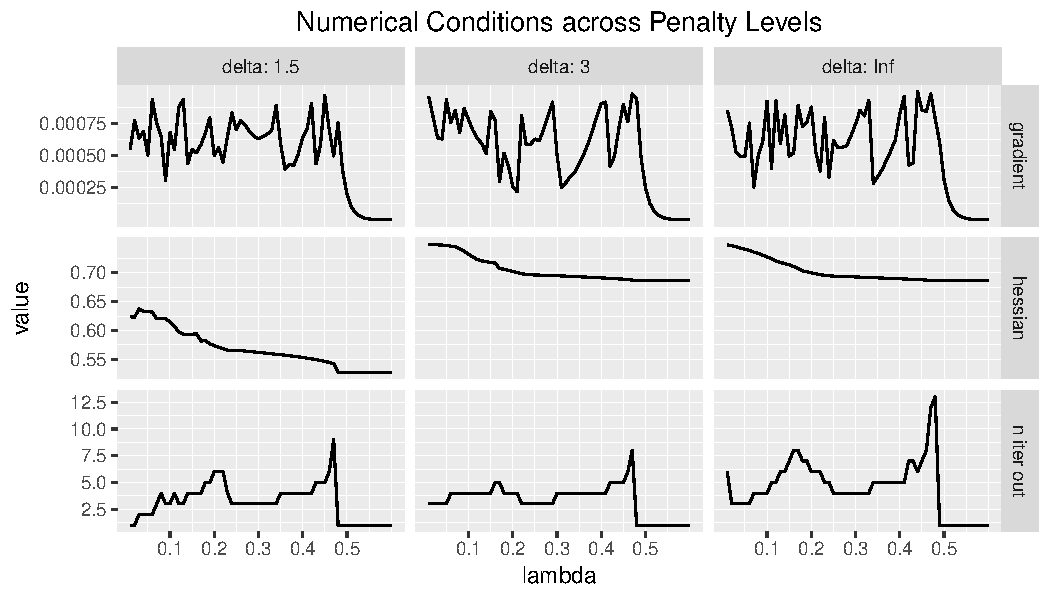
\includegraphics{vignette-lslx-011}
\caption{\label{fig:num_cond}Maximum element of absolute sub-gradient (top), minimum diagonal element of approximated Hessian (middle), and number of iterations (bottom) across all the penalty and convexity levels. }
\end{figure}


The plot-related methods can be used to plot the fitting results stored in an \code{lslx} object. For example, the \code{$plot_numerical_condition()} method displays the numerical conditions for assessing the quality of optimization. It can be called by
\begin{Schunk}
\begin{Sinput}
R> lslx_fa$plot_numerical_condition()
\end{Sinput}
\end{Schunk}

Figure \ref{fig:num_cond} displays how the number of iterations, the maximum element of absolute sub-gradient, and the minimum diagonal element of approximated Hessian change by penalty level and convexity level. We can see that the algorithm converges within a few iterations under all specified penalty and convexity levels, and there are no non-convexity problems (indicated by positive values of all \code{objective Hessian convexity}). Note that the non-convexity problem is detected via an approximated Hessian used in the optimization algorithm, not the exact one. Another useful plotting method is \code{$plot_coefficient()}, which draws solution paths. The following code plots the solution paths of coefficients in the block of \code{y<-f}, i.e., the factor loadings. 
\begin{Schunk}
\begin{Sinput}
R> lslx_fa$plot_coefficient(block = "y<-f")
\end{Sinput}
\end{Schunk}
In Figure \ref{fig:solution_path}, we can observe how the values of loadings change by penalty level and convexity level. Under $\delta=1.5$, MCP shrinks the values of estimates sharply. On the contrary, infinite $\delta$ yields relatively smooth solution paths. 

\begin{figure}[t!]
\centering
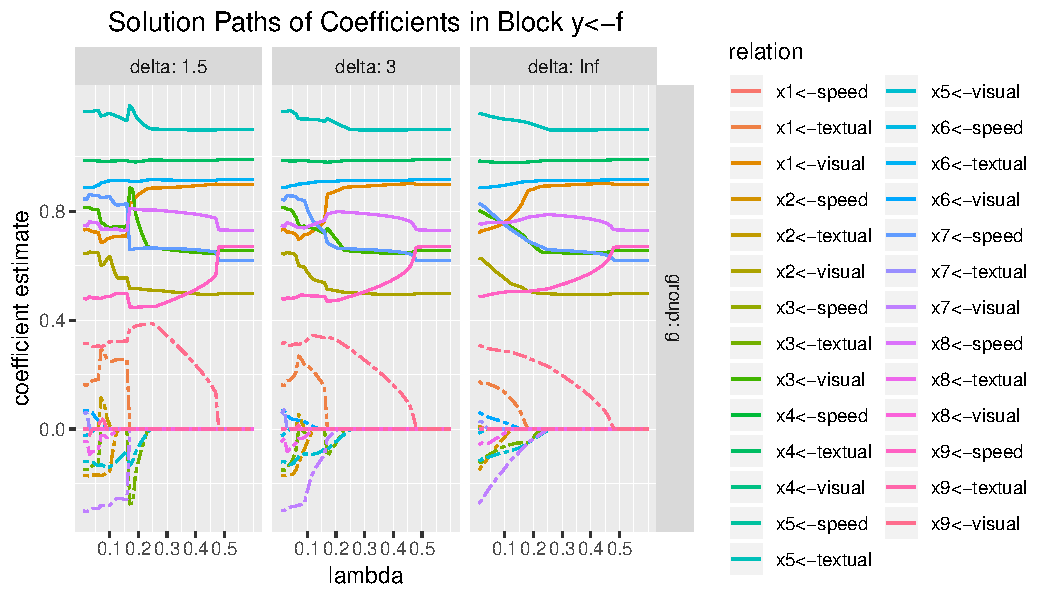
\includegraphics{vignette-lslx-014}
\caption{\label{fig:solution_path}Solution paths of factor loading estimates across all the penalty and convexity levels. Freely estimated and penalized loadings are represented by solid and broken lines, respectively.}
\end{figure}

\subsection{Practical guidelines} \label{sec:lslx_guide}
This subsection discusses several practical issues when using \pkg{lslx}, including the check of model identification, the initialization of $\Lambda$ and $\Delta$, and the choice of selectors.

The first issue is about model identification. In a semi-confirmatory analysis, the specified model is sometimes not identified under the usual SEM framework (e.g., \code{model_fa}). However, PL can still estimate it because the penalty term introduces additional constraints on the penalized parameters. For example, with LASSO the optimization problem in Equation \ref{eq:pl_problem} can be equivalently represented by $\min_{\theta} \mathcal{D}(\theta)$ such that $\sum_{q=1}^Q c_{\theta_q}|\theta_q| \leq \gamma$ for some $\gamma>0$ \citep[see][]{Tibshirani1996}. In fact, PL is often implemented as a solution to overcome the $P>N$ problem (underidentified model) in regression analysis. Despite there is no general rule to ensure the identifiability before PL fitting, it can be checked empirically. Motivated by \cite{Shapiro1983}, the local identifiability of the selected model can be checked by examining whether the smallest singular value of $\frac{\partial \tau(\hat{\theta})}{\partial \vartheta^\top}$ is numerically larger than zero \citep[see also][]{Huang}, where $\hat{\vartheta}$ is a vector formed by the freely estimated and penalized non-zero elements of $\hat{\theta}$, the so-called effective elements of $\hat{\theta}$. For example, our BIC selected factor model can be checked by
\begin{Schunk}
\begin{Sinput}
R> moment_jacobian <- lslx_fa$extract_moment_jacobian(
+    selector = "bic", type = "effective")
R> min(svd(moment_jacobian)$d)
\end{Sinput}
\begin{Soutput}
[1] 0.211
\end{Soutput}
\end{Schunk}
Because the value is evidently larger than zero, we conclude that the selected model is at least locally identified. Note that by default \code{$extract_moment_jacobian()} returns the whole model Jacobian matrix. To only extract the Jacobian with respect to the effective parameters, \code{type = "effective"} should be used. 

The second issue is how to initialize $\Lambda$ and $\Delta$. Despite that \pkg{lslx} automatically initializes them by setting \code{lambda_grid = "default"} and \code{delta_grid = "default"}, the discussion below can help users to understand how \pkg{lslx} works. In linear regression, $\Lambda$ is often initialized by (1) setting $\lambda_1$ as a small number (e.g., $\lambda_1 \approx \log(N)/N$ in \pkg{lslx}) and $\lambda_K$ as a minimal value that shrinks all the penalized parameters to be zero; (2) constructing $K$ values decreasing from $\lambda_K$ to $\lambda_1$ on the log scale \citep[e.g.,][]{Friedman2010}. However, making all penalized parameters to be zero is unnecessary in practice. Let $t$ denote a specified upper bound such that $\lambda_K$ can shrink any standardized and unpenalized $|\tilde{\theta}_q^*| \leq t$ to be zero. Based on the rationale described in Appendix \ref{app:initialize}, $\lambda_K$ can be loosely approximated by 
\begin{equation} \label{eq:lower_bound_lambda}
\lambda_K \approx \frac{\sigma_\text{max}}{ \sigma_\text{min}(1-r_\text{max}^2) }t,
\end{equation}
where $\sigma_\text{min}$ and $\sigma_\text{max}$ are the maximum and minimum standard deviation of both response variables and latent factors, respectively, and $r_\text{max}^2$ is the largest coefficient of determination for endogenous variables. For example, by using $t = 0.3$, $r_\text{max}^2= 0.6$, and $\sigma_\text{max}=\sigma_\text{min}=1$, we have $\lambda_K \approx 0.75$. To initialize $\Delta$, it should be known that a small $\delta$ may result in a non-convexity problem and a too large $\delta$ suffers from the problem of biased estimation. A loose approximation for $\delta_1$, the smallest element of $\Delta$, is
\begin{equation} \label{eq:lower_bound_delta}
\delta_1 \approx \frac{  \sigma_\text{max}^2(1-r_\text{min}^2)}{\sigma_\text{min}^2 },
\end{equation}
where $r_\text{min}^2$ is the smallest coefficient of determination for endogenous variables. The largest element $\delta_L$ is often set as infinity to obtain a LASSO solution, which is used as a warm start for calculating $\hat{\theta}$ under a smaller $\delta$ \citep[see][]{Mazumder2011}. In practice, too small values of $\delta$ often make problematic fitting results (e.g., non-convergence or non-convexity of approximated Hessian matrix). By default, \pkg{lslx} will not use them in \code{$summarize()} or other methods relying on fitting results. To include these problematic results, users should set \code{include_faulty = TRUE}, but it is generally not recommended.

The third issue is the choice of selectors. The information criteria in \pkg{lslx} can be distinguished into three types: AIC-type (AIC and AIC3), BIC-type (BIC and CAIC), and mixed-type (HBIC and ABIC). By their relative orders of $C_N$, it is expected that BIC-type is the most conservative (i.e., it results in the sparsest estimate with the price of lower goodness-of-fit), followed by mixed-type, and then AIC-type which tends to choose a relatively complex model. In theory, a BIC-type criterion asymptotically choose a quasi-true model with probability one \citep[e.g.,][]{Huang2017}. However, under small sample sizes or weak signals, an AIC-type criterion generally yields better selection results \citep[e.g.,][]{Vrieze2012}. The behavior of a mixed-type criterion is also mixed. It performs close to AIC under small sample sizes and becomes similar to BIC asymptotically. Despite a mixed-type criterion might not outperform its competitors in the home field of AIC or BIC (e.g., small sample size or strong signal settings), its overall performance across different conditions is good \citep[e.g.,][]{Lin2017}. If users don't have strong arguments to use an AIC-type or a BIC-type criterion, the author would recommend employing a mixed-type one.



\section{Advanced functionality} \label{sec:adv}
In this section, two advanced functions of \pkg{lslx} are described: the two-stage method with auxiliary variables for handling missing data and the reparameterized multi-group SEM to explore population heterogeneity.


\subsection{Two-stage method for missing data} \label{sec:adv_miss}
When conducting SEM, it is likely to encounter missing values. In \pkg{lslx}, missing values can be handled by the listwise deletion (LD) method and the two-stage (TS) method \citep{Yuan2000}. LD only uses complete observations for further analysis. If the mechanism is missing completely at random \citep[MCAR;][]{Rubin1976}, LD can yield a consistent estimator. However, LD suffers from loss of efficiency because the dropped incomplete cases still carry information for estimation. On the other hand, TS first minimizes the likelihood based on all available observations to calculate saturated moments. The obtained moment estimates are used for subsequent SEM analysis. Under the assumption of missing at random \citep[MAR;][]{Rubin1976}, TS is consistent. In addition, the standard errors of coefficients can be consistently estimated \citep[e.g.,][]{Yuan2008}. Compared with LD, TS is generally valid (in terms of consistency) and more efficient (with respect to mean squared error), thus \pkg{lslx} sets TS as the default. The current version also supports the inclusion of auxiliary variables to make the MAR assumption more plausible \citep{Savalei2009}.

Specifically, let $\mathcal{Y}^o = \{ y_n^o \}_{n=1}^N$ denote an observed random sample with $y_n^o$ being the observed part of $y_n$. The first stage of TS aims to estimate the saturated mean $\mu(\tau)$ and covariance matrix $\Sigma(\tau)$ based on $\mathcal{Y}^o$, where $\tau^\top=(\mu^\top, \sigma^\top)$ is a saturated moment vector with $\sigma = \text{vech}(\Sigma)$. To obtain $\hat{\tau}$, the TS method maximizes the following likelihood function
%
\begin{equation} \label{eq:likelihood_miss}
\mathcal{L}(\tau) = -\frac{1}{2N} \sum_{n=1}^N \log{ \big| \Sigma_n(\tau) \big|} -
\frac{1}{2N} \sum_{n=1}^N [y_n^o - \mu_n(\tau)]^\top \Sigma_n(\tau)^{-1} [y_n^o - \mu_n(\tau)],
\end{equation}
%
where $\mu_n(\tau)$ and $\Sigma_n(\tau)$ are the saturated mean and covariance structure for $y_n^o$. Equation \ref{eq:likelihood_miss} can be optimized by using an expectation-maximization (EM) algorithm \citep{Dempster1977}. In the second stage of TS, Equation \ref{eq:pl_problem} is solved using Algorithm \ref{alg:opt} with $m$ and $S$ replaced by $\mu(\hat{\tau})$ and $\Sigma(\hat{\tau})$, respectively.

One may ask why \pkg{lslx} doesn't implement the so-called full-information (FI) approach to handle missing values \citep{Enders2001d}. The main reason is that the TS method is efficient in terms of computation time. The additional cost introduced by TS is only for calculating $\hat{\tau}$ in the first-stage. In contrast, the FI approach requires an expectation step before each outer iteration \citep{Jamshidian1999}. Additionally, current evidence shows that the FI approach has no particular advantage over TS, both theoretically \citep{Yuan2000} and empirically \citep{Savalei2009, Savalei2014}. 

Now, we demonstrate how to use \pkg{lslx} to conduct TS using the data from \cite{Holzinger1939} again. Because the original data set is complete, missing values are created according to the example of \code{twostage()} in package \pkg{semTools} \citep{semTools}. Missingness in \code{x5} and \code{x9} depends on the values of \code{x1} and \code{age}, respectively.
\begin{Schunk}
\begin{Sinput}
R> data_miss <- lavaan::HolzingerSwineford1939
R> data_miss$x5 <- ifelse(
+    test = data_miss$x1 <= quantile(data_miss$x1, .3), 
+    yes = NA, no = data_miss$x5)
R> data_miss$age <- data_miss$ageyr + data_miss$agemo / 12
R> data_miss$x9 <- ifelse(
+    test = data_miss$age <= quantile(data_miss$age, .3), 
+    yes = NA, no = data_miss$x9)
\end{Sinput}
\end{Schunk}
An \code{lslx} object is initialized with a relatively parsimonious CFA model. To include auxiliary variables, the \code{auxiliary_variable} argument should be declared. 
\begin{Schunk}
\begin{Sinput}
R> model_miss <- "x1 + x2 + x3 <=: visual
+                 x4 + x5 + x6 <=: textual
+                 x7 + x8 + x9 <=: speed
+                 visual  <=> 1 * visual
+                 textual <=> 1 * textual
+                 speed   <=> 1 * speed"
R> lslx_miss <- lslx$new(model = model_miss, data = data_miss,
+    auxiliary_variable = c("ageyr", "agemo"), verbose = FALSE)
\end{Sinput}
\end{Schunk}
In this example, \code{"ageyr"} and \code{"agemo"} are set as auxiliary variables. Since the CFA model may not fit the data well due to its independent cluster structure for loadings, motivated by Bayesian SEM \citep{Muthen2012}, a correlated residuals structure is considered. In fact, PL can be also seen as a maximum of a posteriori (MAP) method under a Bayesian framework \citep[see][]{Meng2008,Strawderman2013}. The \code{$penalize_block()} method can be used to penalize coefficients in a specified block by type
\begin{Schunk}
\begin{Sinput}
R> lslx_miss$penalize_block(block = "y<->y", type = "fixed", verbose = FALSE)
\end{Sinput}
\end{Schunk}
This code sets all coefficients with \code{type = "fixed"} in \code{block = "y<->y"} as penalized. Despite that such a model is not identified under the usual SEM framework, PL can still estimate it. The CFA model with correlated residuals is fitted to the data via the \code{$fit_lasso()} method, which is a convenient wrapper for \code{$fit()} with \code{penalty_method = "lasso"}
\begin{Schunk}
\begin{Sinput}
R> lslx_miss$fit_lasso(verbose = FALSE)
\end{Sinput}
\end{Schunk}
By default, \pkg{lslx} implements the TS method for handling missing data. It can be explicitly set by \code{missing_method = "two_stage"}. If any auxiliary variable is specified when initializing an \code{lslx} object, the variable will be included to estimate the saturated moments. Finally, the robust AIC is utilized to select an optimal penalty level
\begin{Schunk}
\begin{Sinput}
R> lslx_miss$summarize(selector = "raic", style = "minimal")
\end{Sinput}
\begin{Soutput}
General Information                                                 
   number of observations                 301.000
   number of complete observations        138.000
   number of missing patterns               4.000
   number of groups                         1.000
   number of responses                      9.000
   number of factors                        3.000
   number of free coefficients             30.000
   number of penalized coefficients        36.000

Numerical Conditions                                                 
   selected lambda                          0.130
   selected delta                            none
   objective value                          0.168
   objective gradient absolute maximum      0.001
   objective Hessian convexity              0.741
   number of iterations                     2.000
   loss value                               0.051
   number of non-zero coefficients         41.000
   degrees of freedom                      13.000
   robust degrees of freedom               16.173
   scaling factor                           1.244
\end{Soutput}
\end{Schunk}
From the summary with \code{style = "minimal"}, we can see that 11 of the 36 penalized coefficients are identified as non-zero. To see which residual covariances are non-zero, the \code{$extract_coefficient_matrix()} method can be used.
\begin{Schunk}
\begin{Sinput}
R> lslx_miss$extract_coefficient_matrix(selector = "raic", block = "y<->y")
\end{Sinput}
\begin{Soutput}
$g
        x1     x2      x3     x4      x5      x6      x7     x8      x9
x1  0.4735  0.000  0.0000 0.0485 -0.1116  0.0000 -0.0801 0.0000  0.0000
x2  0.0000  1.150  0.1034 0.0000  0.0000  0.0000 -0.1050 0.0000  0.0000
x3  0.0000  0.103  0.8780 0.0000 -0.0791  0.0000  0.0000 0.0000  0.0000
x4  0.0485  0.000  0.0000 0.3875  0.0000  0.0000  0.0793 0.0000  0.0000
x5 -0.1116  0.000 -0.0791 0.0000  0.4103  0.0000  0.0000 0.0000  0.0079
x6  0.0000  0.000  0.0000 0.0000  0.0000  0.3476  0.0000 0.0125 -0.0170
x7 -0.0801 -0.105  0.0000 0.0793  0.0000  0.0000  0.9302 0.2534  0.0000
x8  0.0000  0.000  0.0000 0.0000  0.0000  0.0125  0.2534 0.7189  0.0000
x9  0.0000  0.000  0.0000 0.0000  0.0079 -0.0170  0.0000 0.0000  0.3348
\end{Soutput}
\end{Schunk}
The values of fit indices show that this final model with many residual covariances fits the data very well.
\begin{Schunk}
\begin{Sinput}
R> lslx_miss$extract_fit_index(selector = "raic")
\end{Sinput}
\begin{Soutput}
 rmsea    cfi   nnfi   srmr 
0.0246 0.9972 0.9923 0.0315 
\end{Soutput}
\end{Schunk}
In general, the author doesn't recommend the use of the correlated residuals structure because the specified model is too exploratory and the resulting model may be difficult to interpret.



\subsection{Multi-group SEM analysis}
Multi-group SEM (MGSEM) is often used to examine the heterogeneity of model coefficients across several populations \citep{Joreskog1971,Sorbom1974}. Suppose there are $G$ populations sharing common moment structures $\mu(\cdot)$ and $\Sigma(\cdot)$ but having possibly different values for their model parameter $\theta_g$. Let $\theta_{gq}$ denote the $q^{th}$ component of $\theta_g$. Without loss of generality, we assume that $\theta_{1q}$, $\theta_{2q}$, ..., $\theta_{Gq}$ represent the same element selected from $\alpha$, $\mathrm{B}$, or $\Phi$. Hence, a coefficient $\theta_{gq}$ is said to be homogeneous across the $G$ populations if $\theta_{1q}=\theta_{2q}=...=\theta_{Gq}$. Otherwise, we call $\theta_{gq}$ heterogeneous.


Given a multi-group random sample $\mathcal{Y} = \{ \{y_{gn}\}_{n=1}^{N_g} \}_{g=1}^{G}$, ML estimation tries to obtain $\hat{\theta}_1$, $\hat{\theta}_2$, ..., $\hat{\theta}_G$ by minimizing the following multi-group loss function
%
\begin{equation} \label{eq:mgsem}
\begin{aligned}
\mathcal{D}(\theta) = &  \sum_{g=1}^G w_g \left [\mathrm{tr}(S_g \Sigma(\theta_g)^{-1} )- \mathrm{log}| S_g \Sigma(\theta_g)^{-1}| -P \right] \\
& + \sum_{g=1}^G w_g  (m_g-\mu(\theta_g))^\top \Sigma(\theta_g)^{-1} (m_g-\mu(\theta_g)) ,
\end{aligned}
\end{equation}
%
where $m_g=\frac{1}{N_g}\sum_{n=1}^{N_g} y_{gn}$, $S_g = \frac{1}{N_g}\sum_{n=1}^{N_g} (y_{gn}-m_g)(y_{gn}-m_g)^\top$, and $w_g=\frac{N_g}{N}$ with $N=\sum_{g=1}^G N_g$. To test the homogeneity/heterogeneity of parameters across groups, users may impose equality constraints on coefficients. To evaluate the appropriateness of the constraints, they can perform formal statistical tests or use goodness-of-fit indices.

The current version of \pkg{lslx} cannot impose equality constraints on the model parameters. Therefore, it may seem that it is incapable of examining coefficient homogeneity/heterogeneity. However, by using a reparameterized MGSEM with penalization, \pkg{lslx} can still explore homogeneity/heterogeneity patterns \citep[see][]{Huang2018}. In \pkg{lslx}, each group parameter $\theta_g$ is parameterized as
%
\begin{equation}
\theta_g = \underline{\theta} + \underline{\theta}_g,
\end{equation}
%
where $\underline{\theta}$ is called the reference component and $\underline{\theta}_g$ is called the increment component of group $g$. The meaning of $\underline{\theta}$ and $\underline{\theta}_g$ relies on the choice of the reference group. When there is no reference group, i.e., $\underline{\theta}=0$, $\theta_g$ and $\underline{\theta}_g$ are equivalent. If group $j$ is set as reference, $\underline{\theta}_j$ will be set as zero and $\underline{\theta}_g$ will represent the difference of $\theta_g$ and $\theta_j$, i.e., $\underline{\theta}_g = \theta_g - \theta_j$. Under this setting, $\theta_{gq}$ is homogeneous if and only if $\underline{\theta}_{gq}=0$ for $g=1,2,...,G$ ($g \neq j$). Therefore, we can examine the homogeneity/heterogeneity of $\theta_{gq}$ by exploring the sparsity pattern of $\underline{\theta}_{1q}$, $\underline{\theta}_{2q}$, ..., $\underline{\theta}_{Gq}$.

In \pkg{lslx}, MGSEM analysis is implemented by minimizing a PL criterion composed by the multi-group loss function in Equation \ref{eq:mgsem} and a penalty term as follows 
%
\begin{equation}
\mathcal{R}(\theta, \lambda) = \sum_{q=1}^{Q} c_{\underline{\theta}_{q}}\rho(|\underline{\theta}_{q}|, \lambda)+ \sum_{g=1}^{G} \sum_{q=1}^{Q} c_{\underline{\theta}_{gq}}\rho(|\underline{\theta}_{gq}|, \lambda).
\end{equation}
%
This multi-group optimization problem can also be solved by Algorithm \ref{alg:opt}. After that, the PL estimates over $\Lambda \times \Delta$ are derived, and an optimal pair of $(\lambda, \delta)$ can be chosen by minimizing some information criterion in Equation \ref{eq:ic}. In general, the implementation of semi-confirmatory MGSEM is similar to the single-group case except for the emphasis on the homogeneity/heterogeneity of the coefficients across groups.

The following example shows how to use \pkg{lslx} to examine strong factorial invariance via MCP. A possible initialization for this purpose is
\begin{Schunk}
\begin{Sinput}
R> model_mgfa <- "1 * x1 + x2 + x3 <=: visual 
+                 1 * x4 + x5 + x6 <=: textual
+                 1 * x7 + x8 + x9 <=: speed"
R> lslx_mgfa <- lslx$new(model = model_mgfa,
+    data = lavaan::HolzingerSwineford1939, group_variable = "school",
+    reference_group = "Pasteur", verbose = FALSE)
\end{Sinput}
\end{Schunk}
For simplicity, a commonly used independent cluster structure (i.e., each response is only influenced by one latent factor) is considered here. The model fixes the loadings of \code{x1}, \code{x4}, and \code{x7} at one for scale setting. Argument \code{group_variable} specifies which variable should be used as group label, and \code{reference_group} determines the reference group. Note that since \code{"Pasteur"} is set as the reference group, model parameters in \code{"Grant-White"} are now increment components for representing differences. If argument \code{reference_group} is missing, the reference component will be set to zero, which is equivalent to the usual parameterization of MGSEM. By default, \pkg{lslx} treats all non-trivial model parameters as heterogeneous.

The syntax for specifying a multi-group model is generally similar to that of the single-group model, except that a vectorized prefix can be used. An explicit way to specify the multi-group model is
\begin{Schunk}
\begin{Sinput}
R> model_mgfa <- "c(fix(0), fix(1)) * x1 + x2 + x3 <=: visual 
+                 c(fix(0), fix(1)) * x4 + x5 + x6 <=: textual
+                 c(fix(0), fix(1)) * x7 + x8 + x9 <=: speed"
\end{Sinput}
\end{Schunk}
Here, \code{c(fix(0), fix(1))} is a vectorized prefix that sets the corresponding coefficients to zero and one, respectively. In this example, the first group is \code{"Grant-White"} and the second is \code{"Pasteur"}. This order corresponds to the \code{sort()} result for the group names. Note that the coefficients are set to 1 in \code{"Pasteur"} since \code{"Pasteur"} is the reference group. For \code{"Grant-White"}, the increment component should be restricted to 0 to make the corresponding loadings equal to 1 as desired. If \code{c(fix(0), fix(1))} is replaced by \code{fix(1)}, the \pkg{lslx} parser will still interpret \code{fix(1)} as \code{c(fix(0), fix(1))}. Of course, if the \code{reference_group} argument is not specified, \code{fix(1)} will be interpreted as \code{c(fix(1), fix(1))}, i.e., two corresponding loadings will be set to 1. 

So far, the model specification is still not complete. A measurement satisfies the condition of strong factorial invariance if all loadings and intercepts are homogeneous across the considered groups \citep{Meredith1993}. By default, \pkg{lslx} freely estimates all increment components in \code{"Grant-White"}. To penalize some of them, we can use the \code{$penalize_heterogeneity()} method
\begin{Schunk}
\begin{Sinput}
R> lslx_mgfa$penalize_heterogeneity(block = c("y<-f", "y<-1"), 
+    group = "Grant-White", verbose = FALSE)
\end{Sinput}
\end{Schunk}
The code penalizes every coefficient belonging to block \code{"y<-f"} and \code{"y<-1"} in \code{"Grant-White"} according to its reference component. Since restrictions for loadings and intercepts are imposed, the intercepts of latent factors in \code{"Grant-White"} can be safely estimated
\begin{Schunk}
\begin{Sinput}
R> lslx_mgfa$free_block(block = "f<-1", 
+    group = "Grant-White", verbose = FALSE)
\end{Sinput}
\end{Schunk}
To understand how to impose minimal constraints for identification in multi-group factor analysis, refer to \cite{Millsap2011}. The specified model is now fitted with MCP through the \code{$fit_mcp()} method, a wrapper for \code{$fit()} with \code{penalty_method = "mcp"}
\begin{Schunk}
\begin{Sinput}
R> lslx_mgfa$fit_mcp(verbose = FALSE)
\end{Sinput}
\end{Schunk}
Finally, we display the values of loadings and intercepts to evaluate whether they are invariant under the penalty and convexity level selected by HBIC
\begin{Schunk}
\begin{Sinput}
R> loading <- lslx_mgfa$extract_coefficient_matrix(
+    selector = "hbic", block = "y<-f")
R> intercept <- lslx_mgfa$extract_coefficient_matrix(
+    selector = "hbic", block = "y<-1")
R> loading$"Grant-White" - loading$"Pasteur"
\end{Sinput}
\begin{Soutput}
   visual textual speed
x1      0       0     0
x2      0       0     0
x3      0       0     0
x4      0       0     0
x5      0       0     0
x6      0       0     0
x7      0       0     0
x8      0       0     0
x9      0       0     0
\end{Soutput}
\begin{Sinput}
R> t(intercept$"Grant-White" - intercept$"Pasteur")
\end{Sinput}
\begin{Soutput}
  x1 x2    x3 x4 x5 x6    x7 x8 x9
1  0  0 -0.53  0  0  0 -0.44  0  0
\end{Soutput}
\end{Schunk}
The result shows that the loadings are invariant across the two schools. However, the intercepts of \code{x3} and \code{x7} are different. We conclude that the condition of strong factorial invariance is violated. The measurement only satisfies the condition of weak factorial invariance \citep{Meredith1993}, i.e., only loadings are homogeneous across the two schools.



\section[Numerical comparison with lsl and regsem]{Numerical comparison with \pkg{lsl} and \pkg{regsem}} \label{sec:comparison}
In this section, a numerical comparison between \pkg{lslx} (ver.0.6.1), \pkg{lsl} (ver.0.5.6), and \pkg{regsem} (ver.0.9.2) is reported. So far, no studies have strictly evaluated whether existing packages can reliably find PL estimates for SEM. To this end, the minimum function values obtained by the three packages are compared. In addition, the number of iterations and the computation time are also evaluated to understand the performance aspects of existing algorithms.

A multiple indicators and multiple causes (MIMIC) model \citep{Joreskog1975} with nine indicators ($y_1$ - $y_9$), three latent factors ($f_1$ - $f_3$), and six causes ($x_1$ - $x_6$) is considered. The population model for generating data is presented in Figure \ref{fig:true_model}. Data are generated from a multivariate normal distribution with zero mean and the covariance implied by the model.

\begin{figure}[t!]
\centering
\begin{tikzpicture}[auto,node distance=.5cm,
latent/.style={circle,draw,thick,inner sep=0pt,minimum size=9mm,align=center},
manifest/.style={rectangle,draw,thick,inner sep=0pt,minimum width=9mm, minimum height=6mm},
error/.style={circle,thick, inner sep = 0pt, minimum size=6mm},
paths/.style={->, thick, >=stealth'},
dpaths/.style={->, thick, dashed, >=stealth'},
corr/.style={<->,thick, >=stealth', bend left=60},
]
\node [manifest] (Y1) at (0,0) {$y_1$};
\node [manifest] (Y2) [right= 0.4cm of Y1] {$y_2$};
\node [manifest] (Y3) [right= 0.4cm of Y2] {$y_3$};
\node [manifest] (Y4) [right= 0.4cm of Y3] {$y_4$};
\node [manifest] (Y5) [right= 0.4cm of Y4] {$y_5$};
\node [manifest] (Y6) [right= 0.4cm of Y5] {$y_6$};
\node [manifest] (Y7) [right= 0.4cm of Y6] {$y_7$};
\node [manifest] (Y8) [right= 0.4cm of Y7] {$y_8$};
\node [manifest] (Y9) [right= 0.4cm of Y8] {$y_9$};

\node [manifest] (X1) at (2.6, 5.2) {$x_1$};
\node [manifest] (X2) [right= 0.15cm of X1] {$x_2$};
\node [manifest] (X3) [right= 0.15cm of X2] {$x_3$};
\node [manifest] (X4) [right= 0.15cm of X3] {$x_4$};
\node [manifest] (X5) [right= 0.15cm of X4] {$x_5$};
\node [manifest] (X6) [right= 0.15cm of X5] {$x_6$};

\node [latent] (Eta1) [above=1.7cm of Y2] {$f_1$};
\node [latent] (Eta2) [above=1.7cm of Y5] {$f_2$};
\node [latent] (Eta3) [above=1.7cm of Y8] {$f_3$};


\node [error] (E1) [below=of Y1]{};
\node [error] (E2) [below=of Y2]{};
\node [error] (E3) [below=of Y3]{};
\node [error] (E4) [below=of Y4]{};
\node [error] (E5) [below=of Y5]{};
\node [error] (E6) [below=of Y6]{};
\node [error] (E7) [below=of Y7]{};
\node [error] (E8) [below=of Y8]{};
\node [error] (E9) [below=of Y9]{};


\foreach \va in {Y1, Y2, Y3, Y5}
{
\draw [paths] (Eta1.south) to node { } (\va.north);
}

\foreach \vb in {Y4, Y5, Y6, Y8}
{
\draw [paths] (Eta2.south) to node {} (\vb.north);
}
\foreach \vc in {Y2, Y7, Y8, Y9}
{
\draw [paths] (Eta3.south) to node {} (\vc.north);
}

\foreach \vd in {Eta1}
{
\draw [paths] (X1.south) to node { } (\vd.north);
\draw [paths] (X2.south) to node { } (\vd.north);
\draw [paths] (X3.south) to node { } (\vd.north);
\draw [paths] (X4.south) to node { } (\vd.north);
}
\foreach \vd in {Eta2}
{
\draw [paths] (X2.south) to node { } (\vd.north);
\draw [paths] (X3.south) to node { } (\vd.north);
\draw [paths] (X4.south) to node { } (\vd.north);
\draw [paths] (X5.south) to node { } (\vd.north);
}
\foreach \vd in {Eta3}
{
\draw [paths] (X3.south) to node { } (\vd.north);
\draw [paths] (X4.south) to node { } (\vd.north);
\draw [paths] (X5.south) to node { } (\vd.north);
\draw [paths] (X6.south) to node { } (\vd.north);
}


\draw [paths] (E1.north) to node {} (Y1.south);
\draw [paths] (E2.north) to node {} (Y2.south);
\draw [paths] (E3.north) to node {} (Y3.south);
\draw [paths] (E4.north) to node {} (Y4.south);
\draw [paths] (E5.north) to node {} (Y5.south);
\draw [paths] (E6.north) to node {} (Y6.south);
\draw [paths] (E7.north) to node {} (Y7.south);
\draw [paths] (E8.north) to node {} (Y8.south);
\draw [paths] (E9.north) to node {} (Y9.south);

\node [error] (D1) [right= 0mm of Eta1]{};
\node [error] (D2) [right= 0mm of Eta2]{};
\node [error] (D3) [right= 0mm of Eta3]{};


\draw [paths] (D1.north) to node {}  (Eta1.east);
\draw [paths] (D2.north) to node {}  (Eta2.east);
\draw [paths] (D3.north) to node {}  (Eta3.east);

\draw [corr] (D1.north) to node {} (D2.north);
\draw [corr] (D1.north) to node {} (D3.north);
\draw [corr] (D2.north) to node {} (D3.north);

\foreach \ve in {X2, X3, X4, X5, X6}
{
\draw [corr] (X1.north) to node { } (\ve.north);
}

\foreach \vf in {X3, X4, X5, X6}
{
\draw [corr] (X2.north) to node { } (\vf.north);
}

\foreach \vg in {X4, X5, X6}
{
\draw [corr] (X3.north) to node { } (\vg.north);
}

\foreach \vh in {X5, X6}
{
\draw [corr] (X4.north) to node { } (\vh.north);
}
\draw [corr] (X5.north) to node {} (X6.north);

\end{tikzpicture}
\caption{\label{fig:true_model}The population MIMIC model for generating data includes nine indicators ($y_1$ - $y_9$), three latent factors ($f_1$ - $f_3$), and six causes ($x_1$ - $x_6$). The loadings in the independent cluster part are set to 0.7. Other non-zero loadings are specified as 0.2. The covariances of the residuals of latent factors and the regression coefficients are all set to 0.2. The covariance among causes is specified as 0.3. The values of the residual variances are so chosen that indicators, factors, and causes are all standardized.}
\end{figure}



The numerical comparison is made with different sample sizes (200, 400, 600, and 800) and model specifications (simple and complex). For the simple case, the measurement model is assumed to satisfy an independent cluster structure (i.e., \code{y2<-f3}, \code{y5<-f1}, and \code{y8<-f2} are omitted) with \code{y1}, \code{y4}, and \code{y7} set as anchors. The regression coefficients from causes (\code{x1} - \code{x6}) to factors (\code{f1} - \code{f3}) are all estimated with penalty. Other parameters are set as free or fixed according to the sparsity pattern in Figure \ref{fig:true_model}. For the complex case, the model specification is similar to that of the simple one except that all loadings in the non-independent cluster part are now estimated with penalization.

\begin{figure}[t!]
\centering
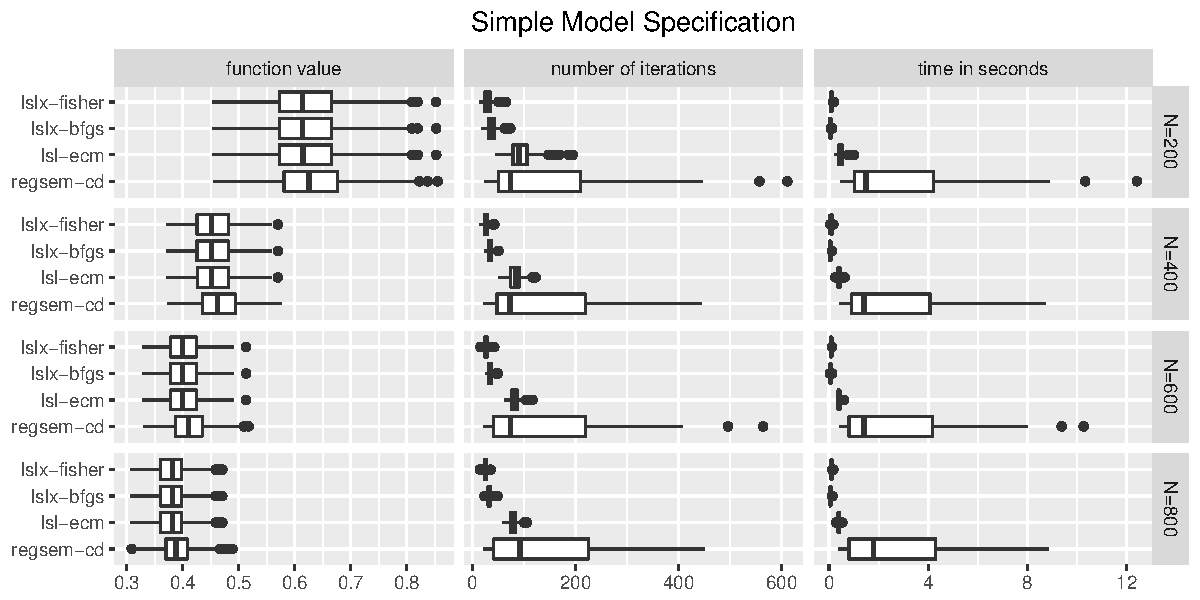
\includegraphics[width=6in]{vignette-lslx-figure-5a.pdf}
\\~\\
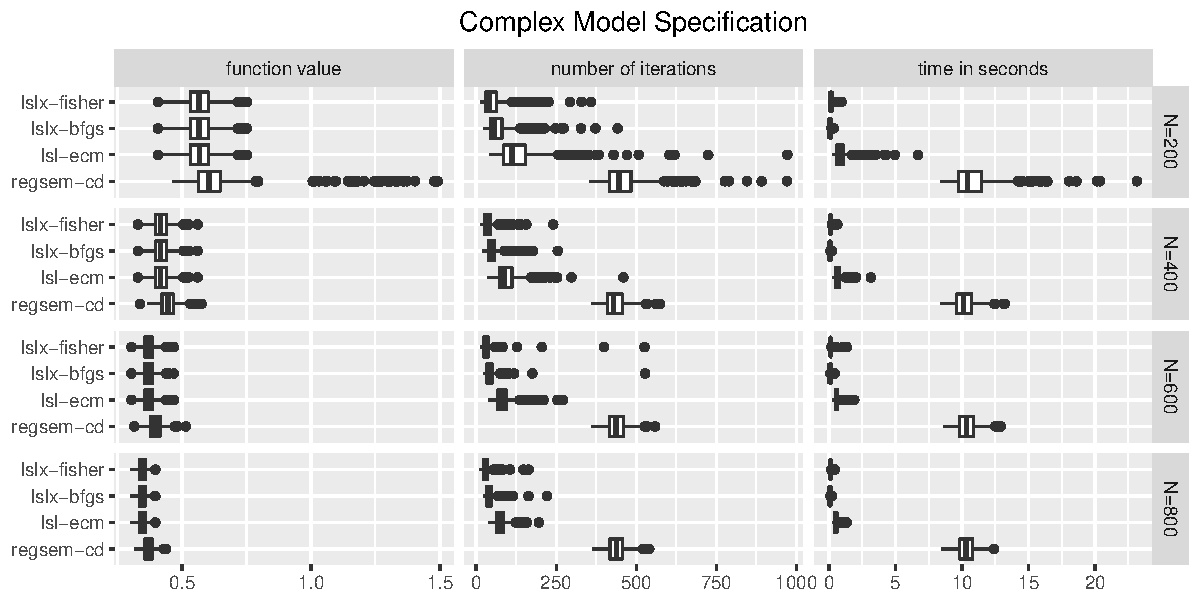
\includegraphics[width=6in]{vignette-lslx-figure-5b.pdf}
\caption{\label{fig:comparison} Boxplots of minimum function values, number of iterations, and computation times in seconds for the four algorithms under different sample sizes (200, 400, 600, and 800) and model specifications (simple and complex). The four algorithms are Fisher scoring, Broyden-Fletcher-Goldfarb-Shanno (BFGS), expectation-conditional maximization (ECM), and coordinate descent (CD).}
\end{figure}




The following five implementations are evaluated: the Fisher scoring (\code{lslx-fisher}) and the Broyden-Fletcher-Goldfarb-Shanno (\code{lslx-bfgs}) from \pkg{lslx}, the expectation-conditional maximization (\code{lsl-ecm}) from \pkg{lsl}, the so-called default (\code{regsem-default}) and the coordinate descent (\code{regsem-cd}) from \pkg{regsem}. The LASSO penalty is implemented with fixed penalty level $\lambda = 0.1$. The maximal number of outer and inner (if needed) iterations is 1000 and 50, respectively. The tolerance is specified as $10^{-5}$, although these packages utilize different rules for assessing convergence. In each condition, the number of replications is set to 500. 

The probabilities of non-convergent samples were first evaluated. Both \pkg{lslx} and \pkg{lsl} yielded nearly minimal non-convergence probabilities. Across all conditions, the probabilities for \code{lslx-fisher} and \code{lslx-bfgs} were 0\% - 0.4\% and 0\% - 1.2\%, respectively. For each condition, \code{lsl-ecm} yielded a perfect convergence rate. On the other hand, \pkg{regsem} produced several incomplete results. The non-convergence probability of \code{regsem-cd} was acceptable between 0.8\% and 13.2\%. However, the probability for \code{regsem-default} was between 43.4\% and 95.6\%. We decided to drop \code{regsem-default} from the rest of the evaluations.

Figure \ref{fig:comparison} shows the comparison results for each condition based on 500 successful replications (with respect to the remaining four algorithms). The minimum function values indicated that \pkg{lslx} and \pkg{lsl} yield similar optimization results. It is interesting to note that the two packages implement conceptually different algorithms. Thus, their consistency cannot be explained by the similarity of the underlying algorithms. However, \pkg{regsem} always yielded larger function values than \pkg{lslx} and \pkg{lsl}. 

As for the number of iterations and the computation time, \code{lslx-fisher} and \code{lslx-bfgs} performed equally well, \code{lsl-ecm} was slower with more iterations, and \code{regsem-cd} was the slowest with the most iterations. Note that the difference in computation time cannot be attributed purely to the nature of algorithms, since the computation cores of \pkg{lsl} and \pkg{regsem} could be speeded up by using compiled code. We observed that \code{lslx-fisher} requires fewer iterations than \code{lslx-bfgs}, but spends similar time to achieve convergence. This is likely due to the difference between the more exact but tedious expected Hessian and the less accurate but simpler BFGS Hessian. 

\section{Conclusions} \label{sec:conclusion}
In this work, an \proglang{R} package \pkg{lslx} is described for semi-confirmatory structural equation modeling (SEM) via penalized likelihood (PL). The package implements a quasi-Newton method to optimize the PL criterion with either LASSO or MCP. To ensure the optimality of the obtained solution, the algorithm checks the first-order condition in each outer iteration. A numerical comparison between competing packages shows that \pkg{lslx} can reliably and efficiently find PL estimates.

Package \pkg{lslx} adopts a \pkg{lavaan}-like syntax for model specification. The current version also offers an \proglang{S3} interface for using \code{lslx} objects, including a wrapper function \code{plsem()} and related \proglang{S3} methods. The author believes that most \pkg{lavaan} users can easily learn to use \pkg{lslx}. The semi-confirmatory SEM is most appropriate when limited substantive theory is available for model specification. Although \pkg{lslx} is not the first package for SEM with PL, it is probably the most sophiscated one in terms of usability, dependability, efficiency, and functionality.

Even though the current version of \pkg{lslx} can fit a wide class of SEM models, there are still limitations. (1) \pkg{lslx} cannot impose linear or non-linear constraints for model parameters. It is worth modifying the current algorithm to incorporate parameter constraints. (2) \pkg{lslx} can only handle an ordinal response by treating it as continuous. However, such an approach is only valid under limited conditions \citep[e.g.,][]{Rhemtulla2012}. Implementing a natural PL method for ordinal SEM could enhance the applicability of the current package. (3) \pkg{lslx} utilizes inference methods assuming that no model selection has been conducted, which may result in inflated Type I error or confidence interval undercoverage. Recent advances in post-selection inference allow making valid inferences even after model selection \citep[e.g.,][]{berk2013, Lee2016}. Future versions of \pkg{lslx} should implement these methods to control the proportion of false positive findings.

\section*{Acknowledgments}
The research was supported in part by Grant MOST 104-2410-H-006-119-MY2 from the Ministry of Science and Technology in Taiwan. The author would like to thank Wen-Hsin Hu for preparing the manuscript.


\bibliography{vignette-lslx}


\newpage

\begin{appendix}
\section{Standard errors and robust degrees of freedom} \label{app:technical}
This appendix describes technical details of computing the standard errors and the so-called robust degrees of freedom in \pkg{lslx}. Let $\hat{\vartheta}$ denote a vector formed by the freely estimated and penalized non-zero elements of PL estimate $\hat{\theta}$. The expected Fisher information matrix under $\hat{\theta}$ is 
\begin{equation}
\widehat{\mathcal{F}} = \left( \frac{\partial \tau(\hat{\theta})}{\partial \vartheta^\top} \right)^\top W(\hat{\theta}) \frac{\partial \tau(\hat{\theta})}{\partial \vartheta^\top}.
\end{equation}
Similarly, the corresponding observed information is
\begin{equation}
\widehat{\mathcal{H}} = \frac{1}{2}
\frac{\partial^2 \mathcal{D}(\hat{\theta})}{\partial \vartheta \partial \vartheta^\top}.
\end{equation}
In \pkg{lslx}, $\widehat{\mathcal{F}}$ is computed via analytical formulas and $\widehat{\mathcal{H}}$ is obtained by numerical differentiation. By inverting $\widehat{\mathcal{F}}$ or $\widehat{\mathcal{H}}$, normal-theory standard errors can be obtained from the diagonal elements of the inverse matrix.

By default, \pkg{lslx} uses a sandwich covariance matrix to construct standard errors. Let $\hat{\tau}$ denote a consistent estimate of population moment vector $\tau$ such that $\sqrt{N}(\hat{\tau} - \tau) \rightarrow \mathcal{N}(0,\Pi)$. If $\hat{\tau}$ is calculated by the method described in Section \ref{sec:adv_miss}, $\Pi$ can be estimated by
\begin{equation}
\widehat{\Pi} = 
\bigg ( 
\frac{\partial^2 \mathcal{L}(\hat{\tau})}{\partial \tau \partial \tau^\top} 
\bigg)^{-1}
\bigg ( 
\frac{1}{N}
\sum_{n=1}^N 
\frac{\partial \mathcal{L}_n(\hat{\tau})}{\partial \tau} 
\frac{\partial \mathcal{L}_n(\hat{\tau})}{\partial \tau^\top}
\bigg )
\bigg ( 
\frac{\partial^2 \mathcal{L}(\hat{\tau})}{\partial \tau \partial \tau^\top} 
\bigg)^{-1},
\end{equation}
where $
\mathcal{L}_n(\tau) = -\frac{1}{2} \log{ \big| \Sigma_n(\tau) \big|} -
\frac{1}{2} [y_n^o - \mu_n(\tau)]^\top \Sigma_n(\tau)^{-1} [y_n^o - \mu_n(\tau)]
$ \citep[e.g.,][]{Yuan2008}. In \pkg{lslx}, the sandwich covariance matrix is obtained by
\begin{equation}
\hat{\mathcal{V}} = 
\widehat{\mathcal{H}}^{-1} 
\frac{\partial \tau(\hat{\theta})}{\partial \vartheta^\top} 
W(\hat{\theta})
\widehat{\Pi}
W(\hat{\theta})
\frac{\partial \tau(\hat{\theta})}{\partial \vartheta} 
\widehat{\mathcal{H}}^{-1}.
\end{equation}
Let $\hat{v}_{ii}$ denote the $i^{th}$ diagonal element of $\hat{\mathcal{V}}$. $\sqrt{\hat{v}_{ii}/N}$ can be used as a standard error for $\hat{\vartheta}_i$, the $i^{th}$ element of $\hat{\vartheta}$. Without the presence of penalization and model selection, the use of $\hat{\mathcal{V}}$ for two-stage estimation can be justified \citep{Yuan2000}.

The robust degrees of freedom is defined as the asymptotic expectation of LR statistics under null hypothesis. The expectation can be approximated by
\begin{equation} \label{eq:df_robust}
df(\hat{\theta}) =
\text{tr} 
\left[ 
\widehat{\Pi} 
\left (
W(\hat{\theta}) - 
W(\hat{\theta}) \frac{\partial \tau(\hat{\theta})}{\partial \vartheta}  \widehat{\mathcal{F}
}^{-1}
\frac{\partial \tau(\hat{\theta})}{\partial \vartheta^{\top}} W(\hat{\theta}) 
\right )
\right ],
\end{equation}
\citep[e.g.,][]{Yuan2007}. This robust degrees of freedom (or equivalent) is often used for model selection with misspecified likelihood \citep[e.g.,][]{Konishi1996, Stone1977, Varin2005}.

\section{PL procedure with elastic net} \label{app:en_algorithm}
To optimize the PL criterion with EN, the first-order optimality condition becomes
%
\begin{equation} \label{eq:optimality_en}
\frac{\partial \mathcal{U}(\hat{\theta}, \lambda)}{\partial \theta_q} \equiv
  \begin{cases}
  \frac{\partial \mathcal{D}(\hat{\theta})}{\partial \theta_q} + \frac{\partial \mathcal{R}_{EN}(\hat{\theta}, \lambda)}{\partial \theta_q}=0 & \quad \text{if }\hat{\theta}_q \neq 0 \text{ or } c_{\theta_q}=0, \\
    \mathrm{sign}(\frac{\partial \mathcal{D}(\hat{\theta})}{\partial \theta_q}) \max \left\{ \big |\frac{\partial \mathcal{D}(\hat{\theta})}{\partial \theta_q} \big | - \lambda \delta, 0 \right\}=0 & \quad \text{if }\hat{\theta}_q = 0 \text{ and } c_{\theta_q}=1. 
  \end{cases}
\end{equation}
%
where $\frac{\partial \mathcal{R}_{EN}(\theta, \lambda)}{\partial \theta_q} = \lambda \left[\mathrm{sign} (\theta_q) \delta + 2 (1-\delta) \theta_q \right] $. The corresponding solution for Equation \ref{eq:coor_problem} is
%
\begin{equation} \label{eq:coor_solution_en}
\hat{z}_q =
\begin{cases}
\frac{ -a -2\lambda(1-\delta)c -\lambda \delta}{b + 2 \lambda (1-\delta)}  & \quad \text{if }  \frac{ -a -2\lambda(1-\delta)c -\lambda \delta}{b + 2 \lambda (1-\delta)}  \geq -c, \\
-c  & \quad \text{otherwise,}  \\
\frac{-a - 2 \lambda (1-\delta) c + \lambda \delta}{b+2 \lambda(1-\delta)}  & \quad \text{if }  \frac{-a - 2 \lambda (1-\delta) c + \lambda \delta}{b+2 \lambda(1-\delta)} \leq -c. \\
  \end{cases}
\end{equation}
%
Based on the work of \cite{tibshirani2012}, we can calculate the degrees of freedom for an EN penalized estimator through Equation \ref{eq:df_robust} with $\widehat{\mathcal{F}}$ replaced by $\widehat{\mathcal{F}} + \frac{\partial^2 \mathcal{R}_{EN}(\theta, \lambda)}{\partial \vartheta \partial \vartheta^\top} $.

\section{Bounds for penalty and convexity level} \label{app:initialize}
This appendix describes how to obtain approximated values of $\lambda_K$ and $\delta_1$ for $\Lambda$ and $\Delta$ initialization. Let $\beta_{ij}$ denote the $(i,j)$ element of $\mathrm{B}$. According to the ECM algorithm for SEM with PL \citep{Huang}, the thresholding rule for $\beta_{ij}$ under MCP is
\begin{equation} \label{eq:threshold}
\hat{\beta}_{ij} =
  \begin{cases}
    \frac{\text{sign}(\tilde{\beta}_{ij}) \max \{|\tilde{\beta}_{ij}| - \hat{w}_{\beta_{ij}} \lambda,0 \} }{1- \tilde{w}_{\beta_{ij}}/\delta}       & \hat{\beta}_{ij} \leq \lambda \delta, \\
    \tilde{\beta}_{ij}  & \tilde{\beta}_{ij} > \lambda \delta,
  \end{cases}
\end{equation}
where $\tilde{\beta}_{ij}$ is the current unpenalized estimate and $ \hat{w}_{\beta_{ij}}$ is a working weight for $\beta_{ij}$. Under uncorrelated residuals, the working weight can be written as $\hat{w}_{\beta_{ij}} = \frac{\hat{\phi}_{i}^2}{c_{j}^2}$, where $\hat{\phi}_{i}^2$ is the current estimate for $\phi_{i}^2$, and $c_{j}^2$ is the $j^{th}$ diagonal element of $C = \mathbb{E}(\frac{1}{N}\sum_{n=1}^N \eta_{n} \eta_{n}^\top |\mathcal{Y}, \hat{\theta})$. 

Let $\mu_i$ and $\sigma_i$ denote the mean and the standard deviation of $\eta_i$, the $i^{th}$ element of $\eta$. The standardized $\tilde{\beta}_{ij}$ can be written as $\tilde{\beta}^{*}_{ij}=\frac{\sigma_j}{\sigma_i} \tilde{\beta}_{ij}$. If we hope to shrink all $| \tilde{\beta}^{*}_{ij}| \leq t$ to be zero, Equation \ref{eq:threshold} indicates $\lambda_K$ should at least satisfy 
\begin{equation} \label{eq:approx_lambda}
\lambda_K \geq \max_{i,j} \frac{  c_{j}^2 \sigma_i}{ \hat{\phi}_{i}^2 \sigma_j} t
\approx \max_{i,j} \frac{  \sigma_j +  \mu_j^2 / \sigma_j}{ \sigma_i(1-r_{i}^2) }t.
\end{equation}
where $r_i^2$ is the coefficient of determination for $\eta_i$. The approximation is based on $c_{j}^2 \approx \sigma_j^2 + \mu_j^2$. For a system such that all exogenous variables are centered, a loose approximation can be obtained by $\lambda_K \approx  \frac{\sigma_\text{max}}{ \sigma_\text{min}(1-r_\text{max}^2) }t$. 

By Equation \ref{eq:threshold}, $1 - \hat{w}_{\beta_{ij}}/\delta$ must be larger than zero. Therefore, $\delta_1$ can be approximated by
\begin{equation} \label{eq:approx_delta}
\delta_1 \geq \max_{i,j} \frac{ \hat{\phi}_{i}^2 }{c_{j}^2} \approx \max_{i,j} \frac{  \sigma_i^2(1-r_{i}^2)}{ \sigma_j^2 +\mu_j^2 }.
\end{equation}
Again, without the consideration of $\mu_j$, we can loosely use $\delta_1 \approx \frac{  \sigma_\text{max}^2(1-r_\text{min}^2)}{\sigma_\text{min}^2 }$.

In principle, \pkg{lslx} initializes $\Lambda$ and $\Delta$ based on the approximations in Equations $\ref{eq:approx_lambda}$ and \ref{eq:approx_delta}. When variable scales are all the same, these approximations become very simple. Hence, standardization is a good strategy to simplify the initialization problem. Note that the approximations can be further improved if exogenous and endogenous variables are distinguished. However, how to obtain good estimates for $\sigma_{i}^2$ and $r_i^2$ without actual model fitting is still a challenging task. 

\end{appendix}

\end{document}
